\section{Eksperimentalna evaluacija i diskusija rezultata}
\label{chap:eksperimenti}

U ovom poglavlju detaljno se opisuje eksperimentalni postav, provedba eksperimenata te dubinska analiza i interpretacija dobivenih rezultata. Cilj je bio empirijski validirati predloženi hibridni model, kvantificirati njegove performanse i usporediti ga s drugim relevantnim pristupima kako bi se donijeli utemeljeni zaključci o njegovoj primjenjivosti.

\subsection{Postavke okruženja i testni podaci}
Svi eksperimenti provedeni su u programskom okruženju \textbf{Python (verzija 3.x)} na standardnom osobnom računalu. Kako bi se osigurala ponovljivost i kontrolirani uvjeti, za potrebe istraživanja generiran je sintetički skup podataka koji oponaša realističan projektni portfelj. U ovisnosti o eksperimentalnoj seriji, broj jedinstvenih projektnih aktivnosti varirao je od 10 do 100. Svaka aktivnost je parametrizirana slučajnim vrijednostima unutar zadanih raspona, uključujući \textbf{Trošak (\texttt{cost}):} slučajna cjelobrojna vrijednost između 50 i 200, \textbf{ROI (\texttt{roi}):} slučajna decimalna vrijednost između 1.0 i 3.0, i \textbf{Procjene trajanja:} optimistično (između 5 i 10 dana), najvjerojatnije (između 10 i 20 dana) i pesimistično (između 20 i 40 dana).
Ukupni raspoloživi budžet za portfelj (\texttt{BUDGET}) bio je skaliran u skladu sa složenošću problema.

\subsection{Eksperimentalni dizajn}
Kako bi se osigurala metodološka ispravnost i izbjegli proizvoljni zaključci, istraživanje je provedeno kroz dvo-fazni eksperimentalni proces:
\begin{itemize}
    \item \textbf{Faza 1: Analiza i kalibracija genetskog algoritma.} U prvoj fazi provedena je detaljna ablacijska studija kako bi se utvrdilo koji parametri genetskog algoritma daju najkvalitetnija i najstabilnija rješenja za reprezentativni tip problema (50 aktivnosti). Cilj je bio pronaći ``šampionsku'' konfiguraciju GA.
    \item \textbf{Faza 2: Usporedna analiza optimizacijskih modela.} U drugoj fazi, ``šampionska'' konfiguracija GA, dobivena u prvoj fazi, korištena je kao osnova za provođenje konačne usporedbe triju različitih optimizacijskih scenarija i evaluaciju glavnih hipoteza rada na problemima različite skale i restriktivnosti.
\end{itemize}

\subsubsection{Istraživačke hipoteze}
Na temelju teorijske podloge i postavljenih istraživačkih pitanja iz Uvoda, definirane su sljedeće tri glavne hipoteze koje se provjeravaju kroz eksperimente:

\begin{description}
    \item[H1 (Hipoteza o Skalabilnosti):] Povećanjem složenosti problema (broja aktivnosti), performanse modela temeljenog na nasumičnoj pretrazi (Random Search) će se značajno smanjiti u usporedbi s modelima temeljenim na genetskim algoritmima.
    \item[H2 (Hipoteza o Kompromisu):] Hibridni `GA+MC` model će, za razliku od klasičnog `GA (samo ROI)` modela, uspješno identificirati rješenja koja predstavljaju superioran kompromis između profitabilnosti (ROI) i rizika (trajanje projekta), posebno na problemima veće složenosti.
    \item[H3 (Hipoteza o Utjecaju Ograničenja):] Restriktivnost problema, specifično kroz promjenu raspoloživog budžeta, značajno utječe na performanse i stabilnost optimizacijskih modela, pri čemu se očekuje da će ekstremna ograničenja predstavljati najveći izazov za najsloženije modele.
\end{description}

\subsection{Eksperiment 1: Analiza parametara i kalibracija genetskog algoritma}

Prvi eksperiment imao je za cilj empirijski provjeriti utjecaj osnovnih genetskih operatora i parametara na performanse algoritma te odabrati optimalnu konfiguraciju za daljnje testiranje. U tu svrhu provedena je ablacijska studija s pet različitih konfiguracija, gdje je svaka pokrenuta 10 puta (\texttt{RUNS = 10}) radi statističke pouzdanosti. Testirane konfiguracije su bile: \emph{Standardni GA}, \emph{Bez mutacije}, \emph{Bez križanja}, \emph{Više generacija} i \emph{Veća populacija}.

\subsubsection{Rezultati i diskusija} Rezultati ablacijske studije prikazani su u Tablici~\ref{tab:ga_ablation} te grafički na Slici~\ref{fig:ga_ablation}.

\begin{table}[H]
    \centering
    \caption{Rezultati ablacijske studije za parametre GA.}
    \label{tab:ga_ablation}
    \begin{tabular}{|l|c|c|c|c|}
        \hline
        \textbf{Postavka} & \textbf{ROI\_mean} & \textbf{ROI\_std} & \textbf{Trajanje\_mean} & \textbf{Trajanje\_std} \\
        \hline
        Standardni GA & 28.985 & 1.543 & 199.216 & 10.691 \\
        Bez mutacije & 27.627 & 1.581 & 193.497 & 11.364 \\
        Bez križanja & 25.884 & 1.865 & 191.514 & 9.174 \\
        Više generacija & 31.183 & 0.928 & 205.026 & 13.649 \\
        \textbf{Veća populacija} & \textbf{31.683} & \textbf{0.720} & \textbf{213.694} & \textbf{5.574} \\
        \hline
    \end{tabular}
\end{table}

Analiza rezultata potvrđuje obje početne hipoteze i ključnu ulogu genetskih operatora. Uklanjanje križanja drastično smanjuje performanse, potvrđujući da je rekombinacija dobrih rješenja ključan mehanizam pretrage. S druge strane, povećanje računalnih resursa, bilo kroz više generacija (dubina pretrage) ili veću populaciju (širina pretrage), dovodi do superiornih i statistički stabilnijih rješenja. Konfiguracija \emph{Veća populacija} pokazala se najboljom, ostvarivši najviši prosječni ROI uz najnižu standardnu devijaciju. Zanimljivo je primijetiti da konfiguracije s najvišim ROI-em rezultiraju i najdužim prosječnim trajanjem, što stvara prirodni kompromis (\emph{trade-off}) između profita i rizika, koji će biti predmet analize u sljedećem eksperimentu.

\begin{figure}[H]
    \centering
    \begin{subfigure}[b]{0.48\textwidth}
        \centering
        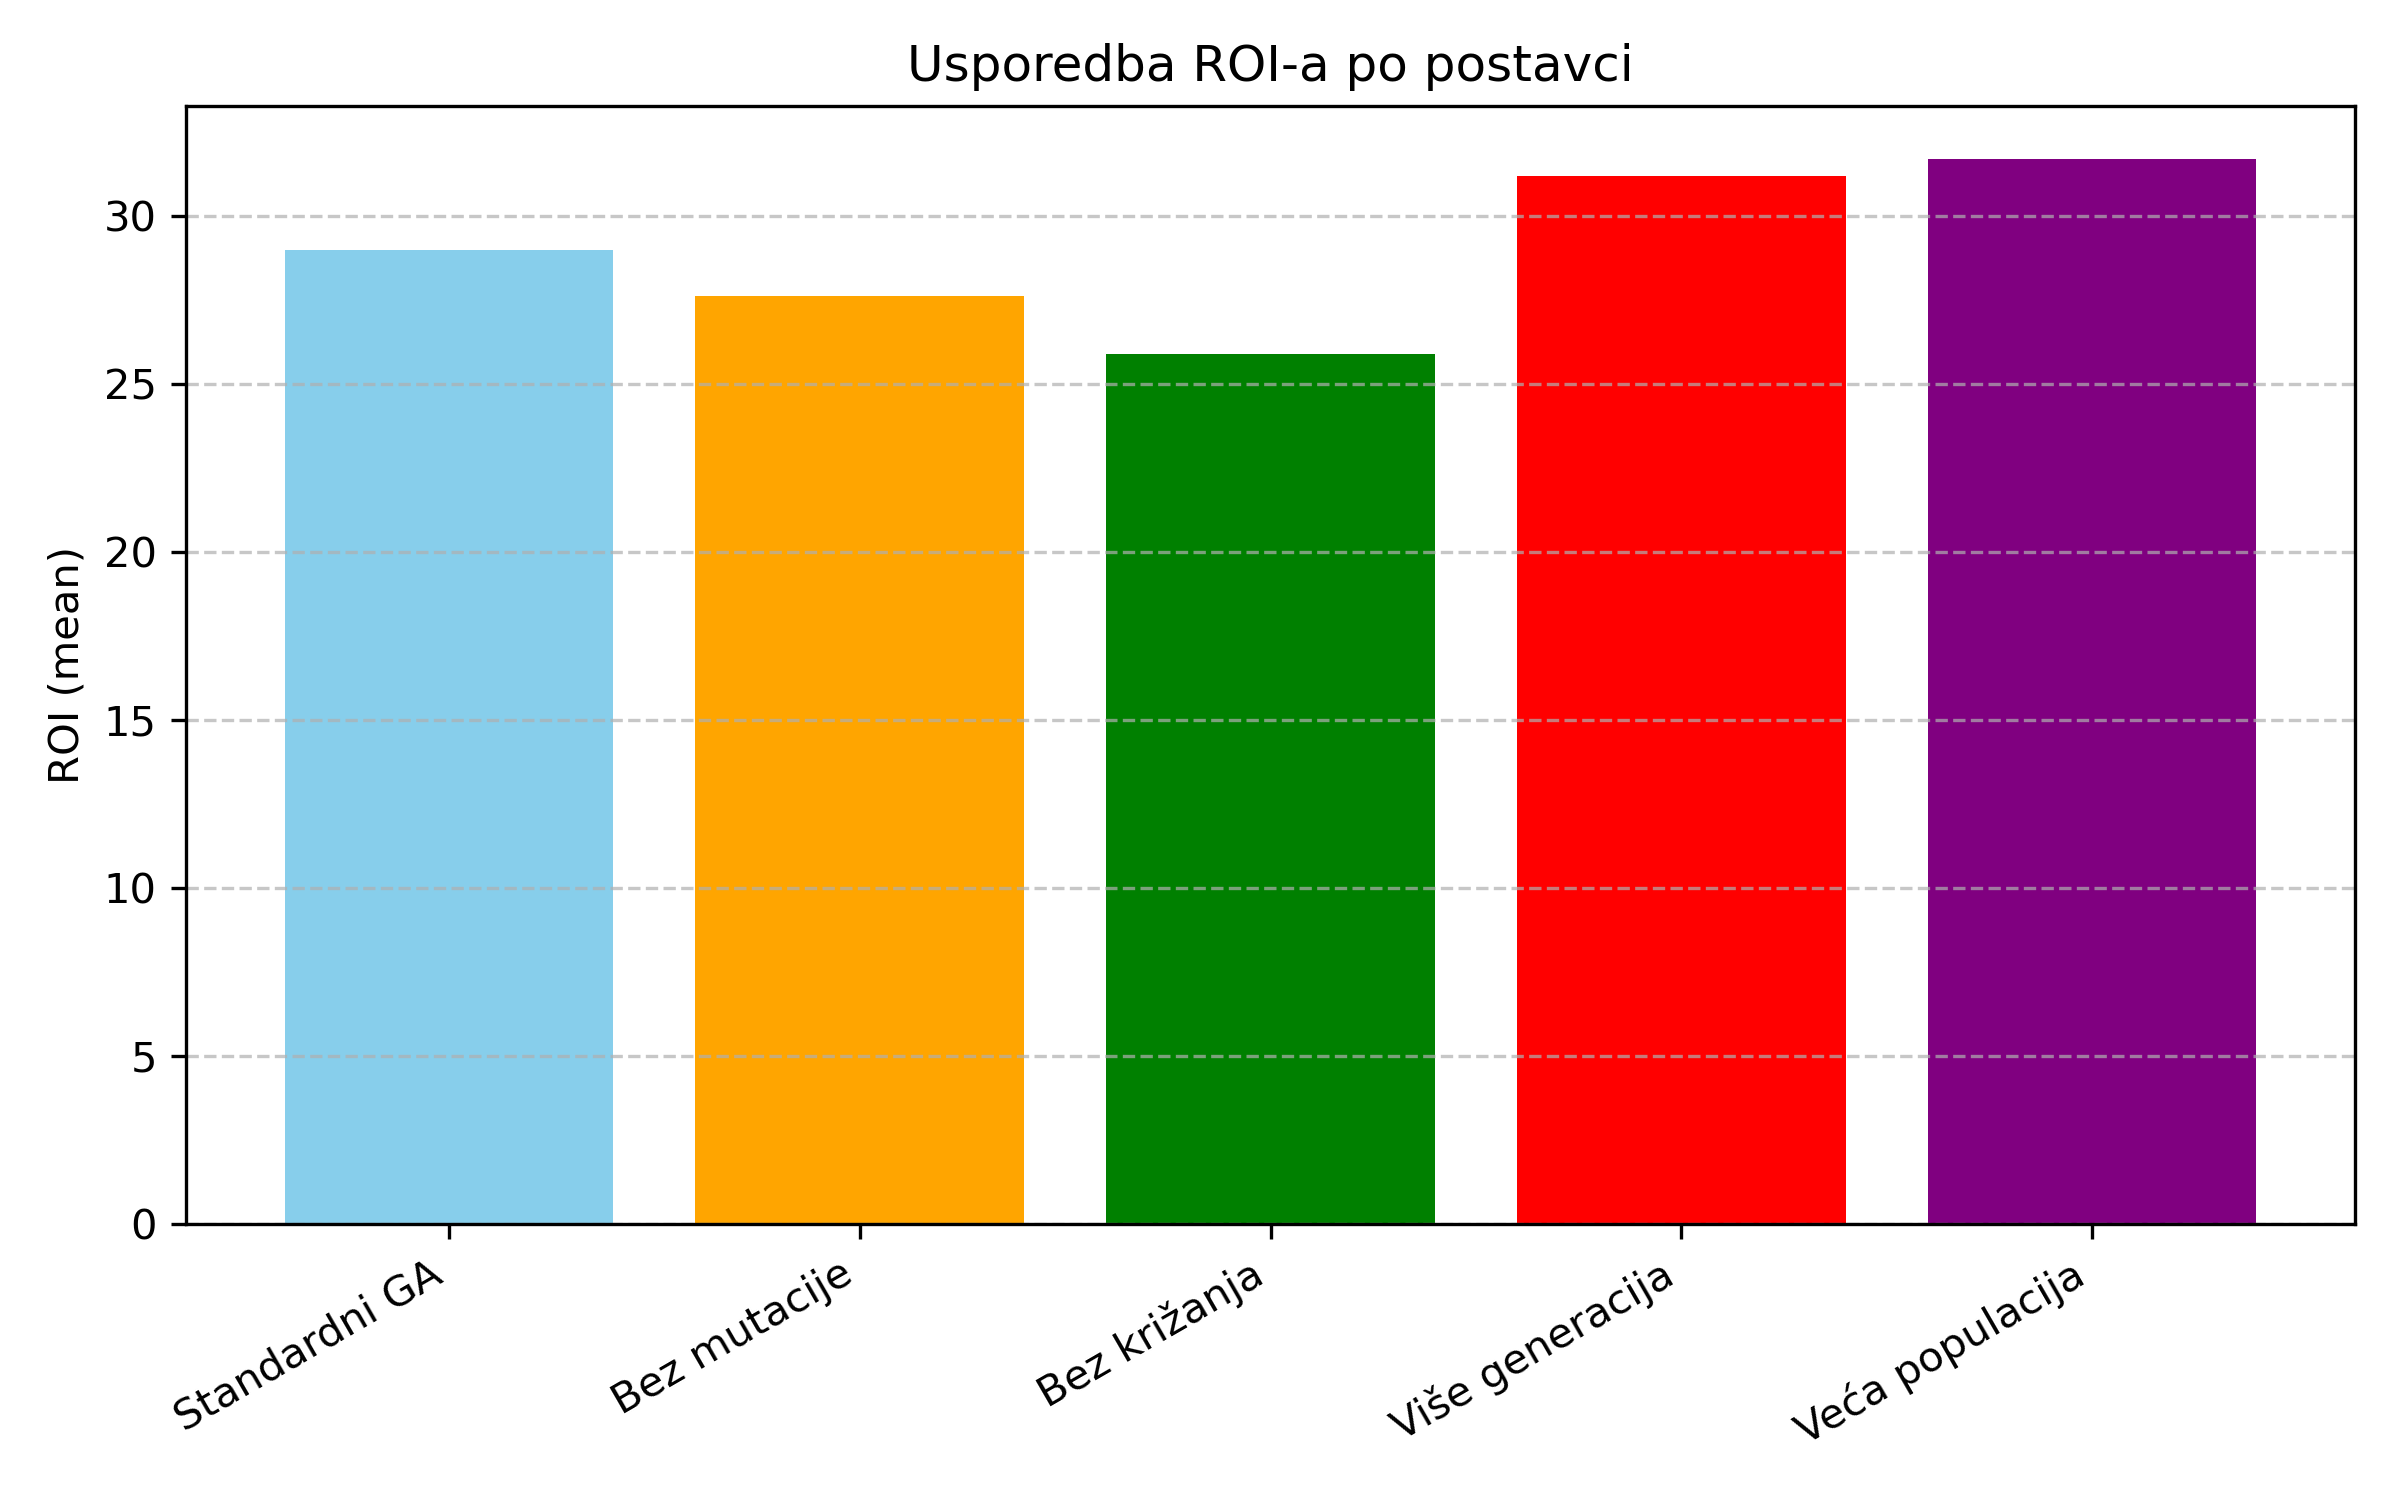
\includegraphics[width=\textwidth]{slike/ga_usporedba_roi.png}
        \caption{Usporedba prosječnog ROI-a.}
        \label{fig:ga_roi}
    \end{subfigure}
    \hfill
    \begin{subfigure}[b]{0.48\textwidth}
        \centering
        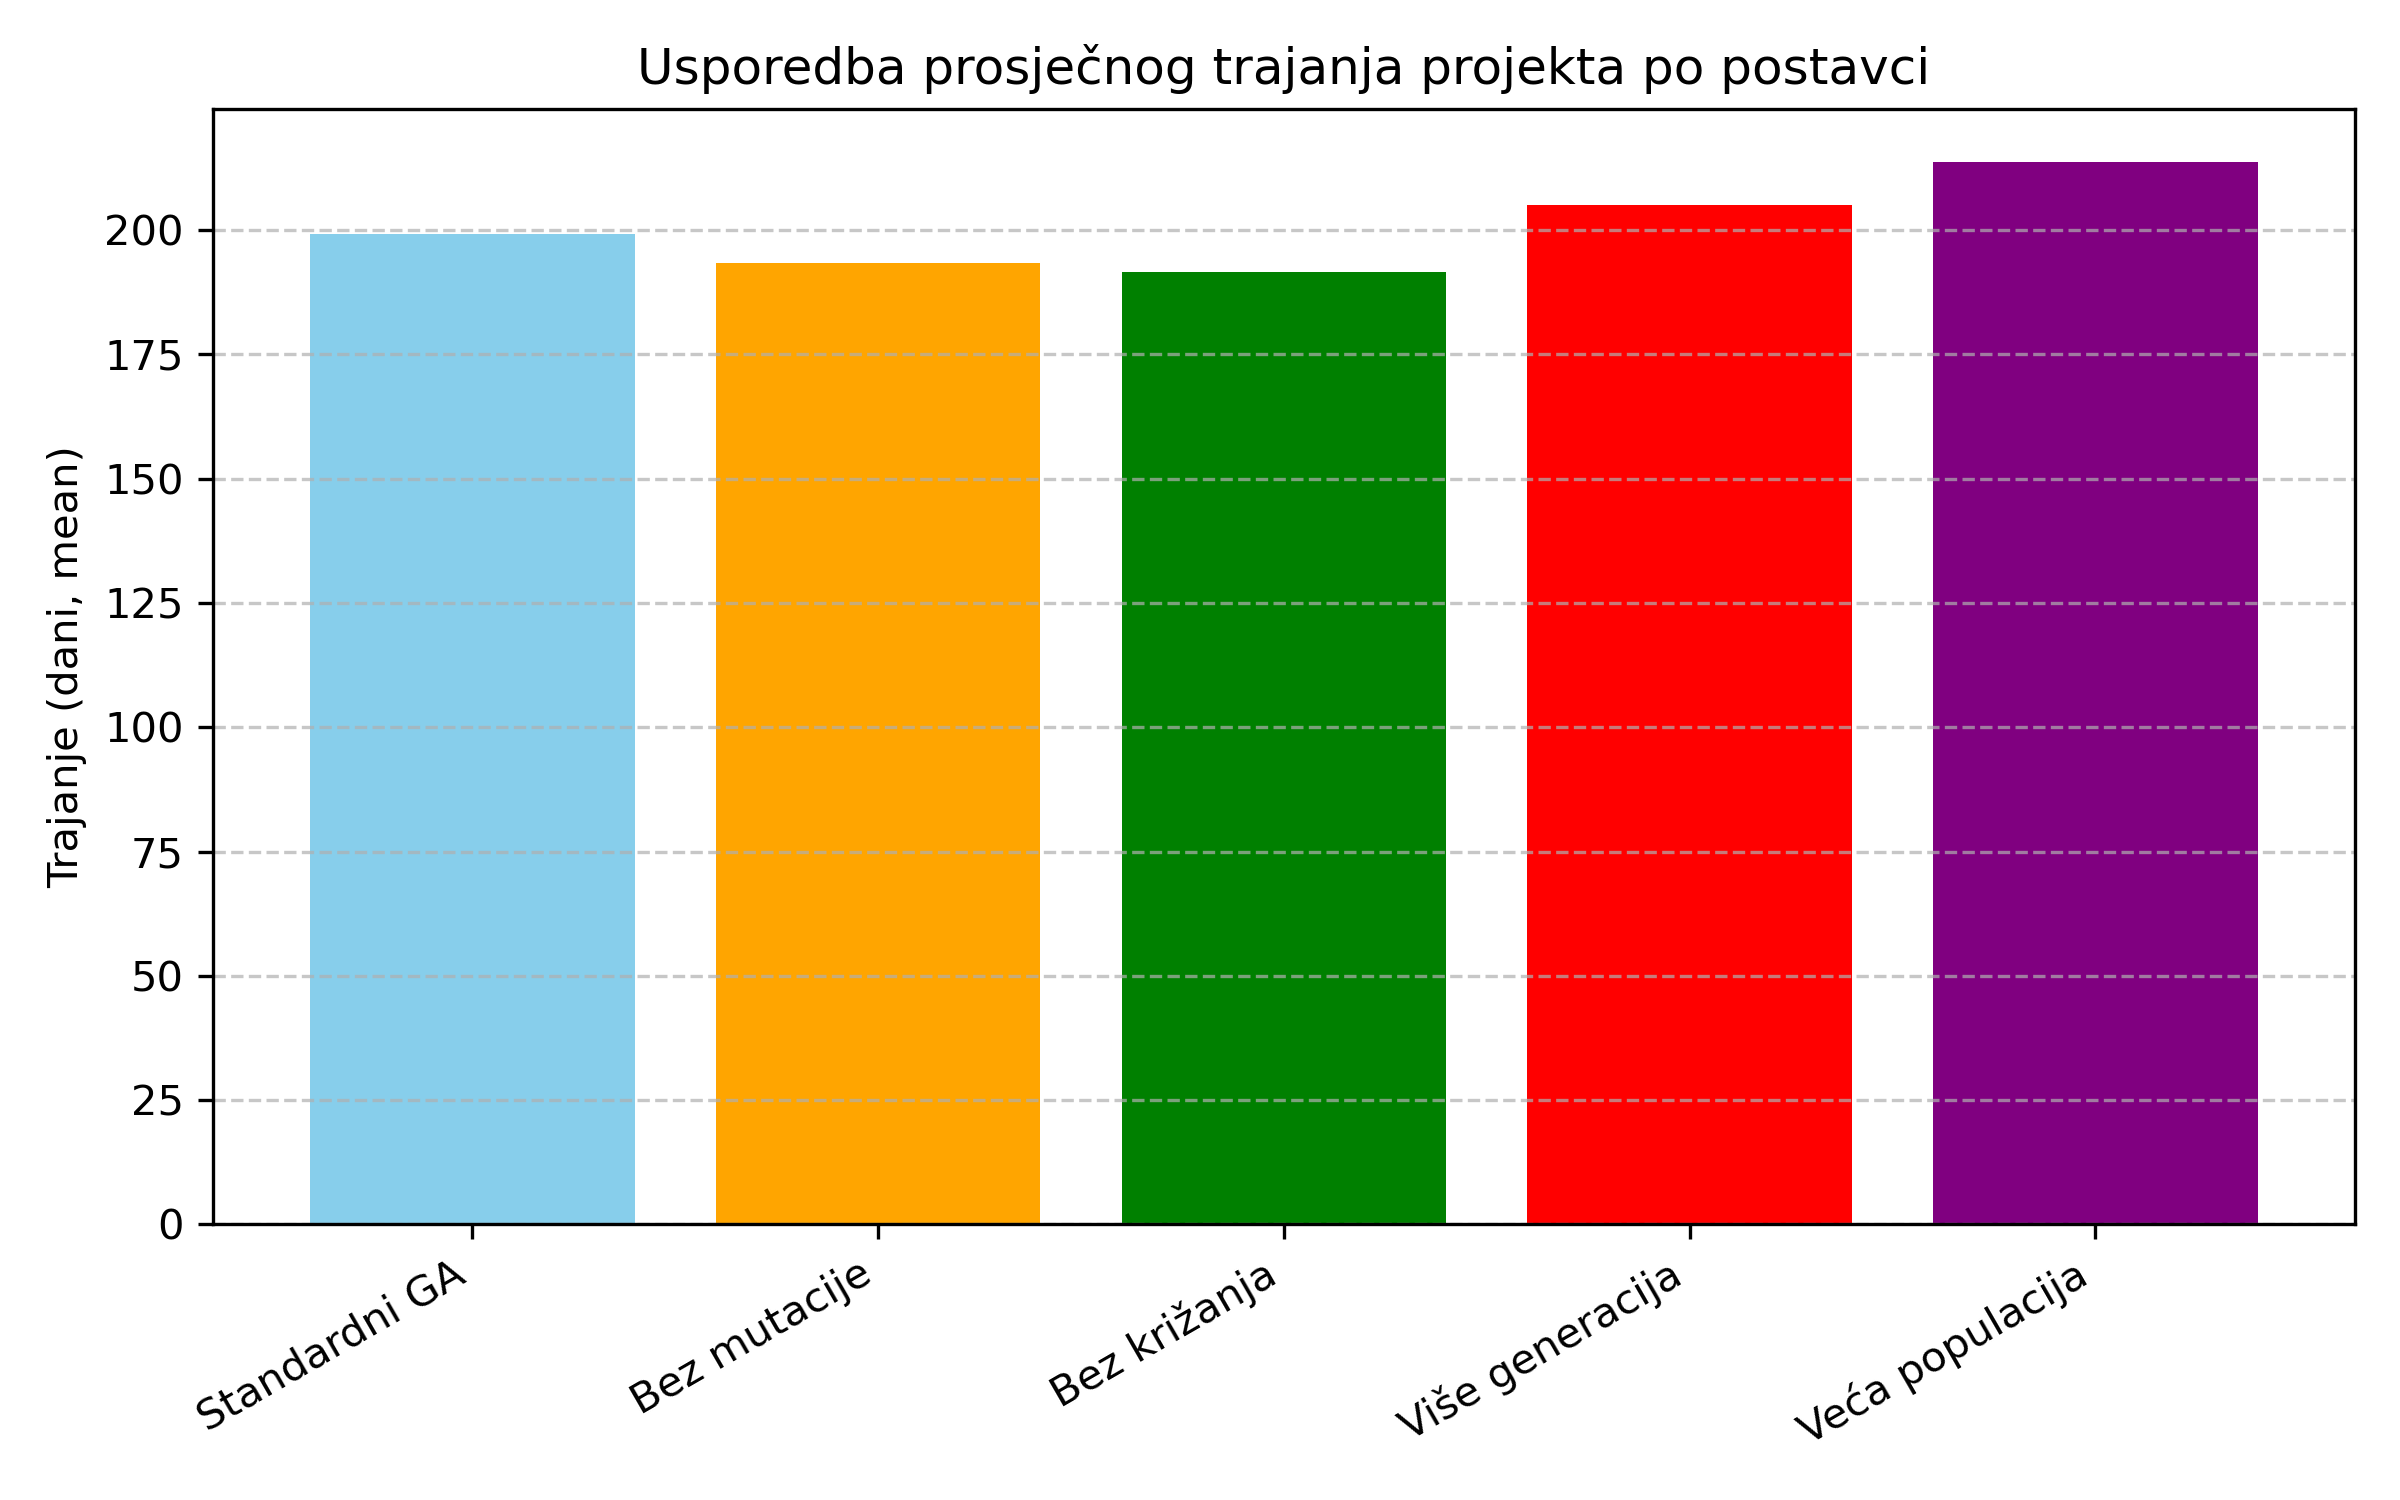
\includegraphics[width=\textwidth]{slike/ga_usporedba_trajanje.png}
        \caption{Usporedba prosječnog trajanja.}
        \label{fig:ga_trajanje}
    \end{subfigure}
    \caption{Grafički prikaz rezultata ablacijske studije za genetski algoritam.}
    \label{fig:ga_ablation}
\end{figure}

Na temelju empirijskih rezultata, konfiguracija \emph{Veća populacija} odabrana je kao ``šampionska''. Njezini parametri (\texttt{POP\_SIZE = 200}, \texttt{NGEN = 40}, itd.) poslužili su kao osnova za definiranje parametara u drugoj fazi istraživanja, uz nužne prilagodbe resursa s obzirom na složenost problema.

\subsection{Eksperiment 2: Usporedna analiza optimizacijskih modela}
Druga faza istraživanja čini ključnu eksperimentalnu provjeru glavne hipoteze rada. Koristeći kalibrirane parametre iz Eksperimenta 1, provedena je sustavna usporedba triju razvijenih modela. Cilj drugog eksperimenta je empirijski provjeriti postavljene istraživačke hipoteze (h1, h2, h3) kroz sustavnu usporedbu performansi, robusnosti i stabilnosti triju razvijenih modela: nasumične pretrage, jedno-kriterijskog GA i više-kriterijskog hibridnog GA+MC modela. usporedba je provedena na problemima različite skale i restriktivnosti prema planu definiranom u tablici~\ref{tab:plan_eksperimenata}. svaki od pet jedinstvenih eksperimentalnih scenarija pokrenut je 10 puta (\texttt{RUNS = 10}) radi osiguravanja statističke pouzdanosti. modeli koji koriste genetski algoritam (`GA (samo ROI)` i `GA+MC (NSGA-II)`) temeljili su se na ``šampionskoj'' konfiguraciji utvrđenoj u eksperimentu 1, uz skaliranje parametra `NGEN` sukladno složenosti problema.

\begin{table}[H]
    \centering
    \caption{Plan naprednih eksperimenata.}
    \label{tab:plan_eksperimenata}
    \resizebox{\textwidth}{!}{
    \begin{tabular}{|l|l|l|l|l|}
        \hline
        \textbf{Eksperiment} & \textbf{NUM\_ACTIVITIES} & \textbf{BUDGET} & \textbf{Pripada seriji} & \textbf{Napomena} \\
        \hline
        A1 & 10 & 1000 & A & Osnovna složenost \\
        \hline
        A2 / B2 & 50 & 2500 & A, B & Centralni / Referentni eksperiment \\
        \hline
        A3 & 100 & 5000 & A & Visoka složenost \\
        \hline
        B1 & 50 & 1500 & B & Restriktivan budžet \\
        \hline
        B3 & 50 & 4000 & B & Labav budžet \\
        \hline
    \end{tabular}
    }
\end{table}

\subsubsection{Rezultati i diskusija}
Svi rezultati dobiveni provođenjem Eksperimenta 2 sažeti su u Tablici~\ref{tab:rezultati}. U nastavku slijedi detaljna diskusija ovih rezultata, organizirana po tematskim cjelinama koje odgovaraju postavljenim hipotezama. Ova tablica predstavlja temelj za daljnju diskusiju.

\begin{table}[H]
    \centering
    \caption{Konačni rezultati usporedne analize optimizacijskih modela.}
    \label{tab:rezultati}
    \resizebox{\textwidth}{!}{
    \begin{tabular}{|l|l|c|c|c|c|}
        \hline
        \textbf{Eksperiment} & \textbf{Scenarij} & \textbf{ROI\_mean} & \textbf{ROI\_std} & \textbf{Trajanje\_mean} & \textbf{Trajanje\_std} \\
        \hline
        A1\_Osnovni & Random Search (MC) & 17.140 & 3.55e-15 & 144.151 & 0.911 \\
        A1\_Osnovni & GA (samo ROI) & 17.140 & 3.55e-15 & 143.103 & 1.239 \\
        A1\_Osnovni & GA+MC (NSGA-II) & 17.140 & 3.55e-15 & 142.003 & 0.372 \\
        \hline
        A2\_Srednji & Random Search (MC) & 40.108 & 0.703 & 341.024 & 9.405 \\
        A2\_Srednji & GA (samo ROI) & 46.125 & 0.412 & 363.632 & 7.843 \\
        A2\_Srednji & GA+MC (NSGA-II) & 44.099 & 0.980 & 319.210 & 13.171 \\
        \hline
        A3\_Slozeni & Random Search (MC) & 95.835 & 1.468 & 715.604 & 10.451 \\
        A3\_Slozeni & GA (samo ROI) & 114.224 & 0.891 & 792.300 & 11.933 \\
        A3\_Slozeni & GA+MC (NSGA-II) & 109.095 & 2.008 & 681.565 & 21.733 \\
        \hline
        B1\_Restriktivan & Random Search (MC) & 24.120 & 1.846 & 197.621 & 20.181 \\
        B1\_Restriktivan & GA (samo ROI) & 37.976 & 0.567 & 253.562 & 12.386 \\
        B1\_Restriktivan & GA+MC (NSGA-II) & 17.711 & 17.728 & 50104.382 & 49894.619 \\
        \hline
        B3\_Labav & Random Search (MC) & 71.379 & 1.114 & 536.901 & 16.247 \\
        B3\_Labav & GA (samo ROI) & 79.065 & 0.518 & 562.191 & 9.345 \\
        B3\_Labav & GA+MC (NSGA-II) & 76.949 & 0.487 & 526.612 & 10.602 \\
        \hline
    \end{tabular}
    }
\end{table}

Dobiveni rezultati analizirani su kroz tematske cjeline, s ciljem odgovaranja na postavljena istraživačka pitanja.

\textbf{Analiza Skalabilnosti (Serija A)}
Kao što je vidljivo na Slici~\ref{fig:a_skalabilnost}, porast složenosti problema drastično utječe na performanse modela. Jaz u \textbf{ROI\_mean} vrijednostima eksponencijalno raste u korist genetskih algoritama, potvrđujući hipotezu o nužnosti inteligentne pretrage (H1). Ovakav nalaz, gdje metaheuristički pristupi značajno nadmašuju nasumičnu pretragu na složenim problemima, u skladu je s rezultatima koje su dobili i drugi istraživači u srodnim domenama primjene \cite{Gandomi2013}. Istovremeno, analiza trajanja otkriva postojanje kompromisa: hibridni model GA+MC (NSGA-II) konzistentno identificira rješenja sa značajno nižim prosječnim trajanjem, potvrđujući hipotezu H2.

\begin{figure}[H]
    \centering
    \begin{subfigure}[b]{0.48\textwidth}
        \centering
        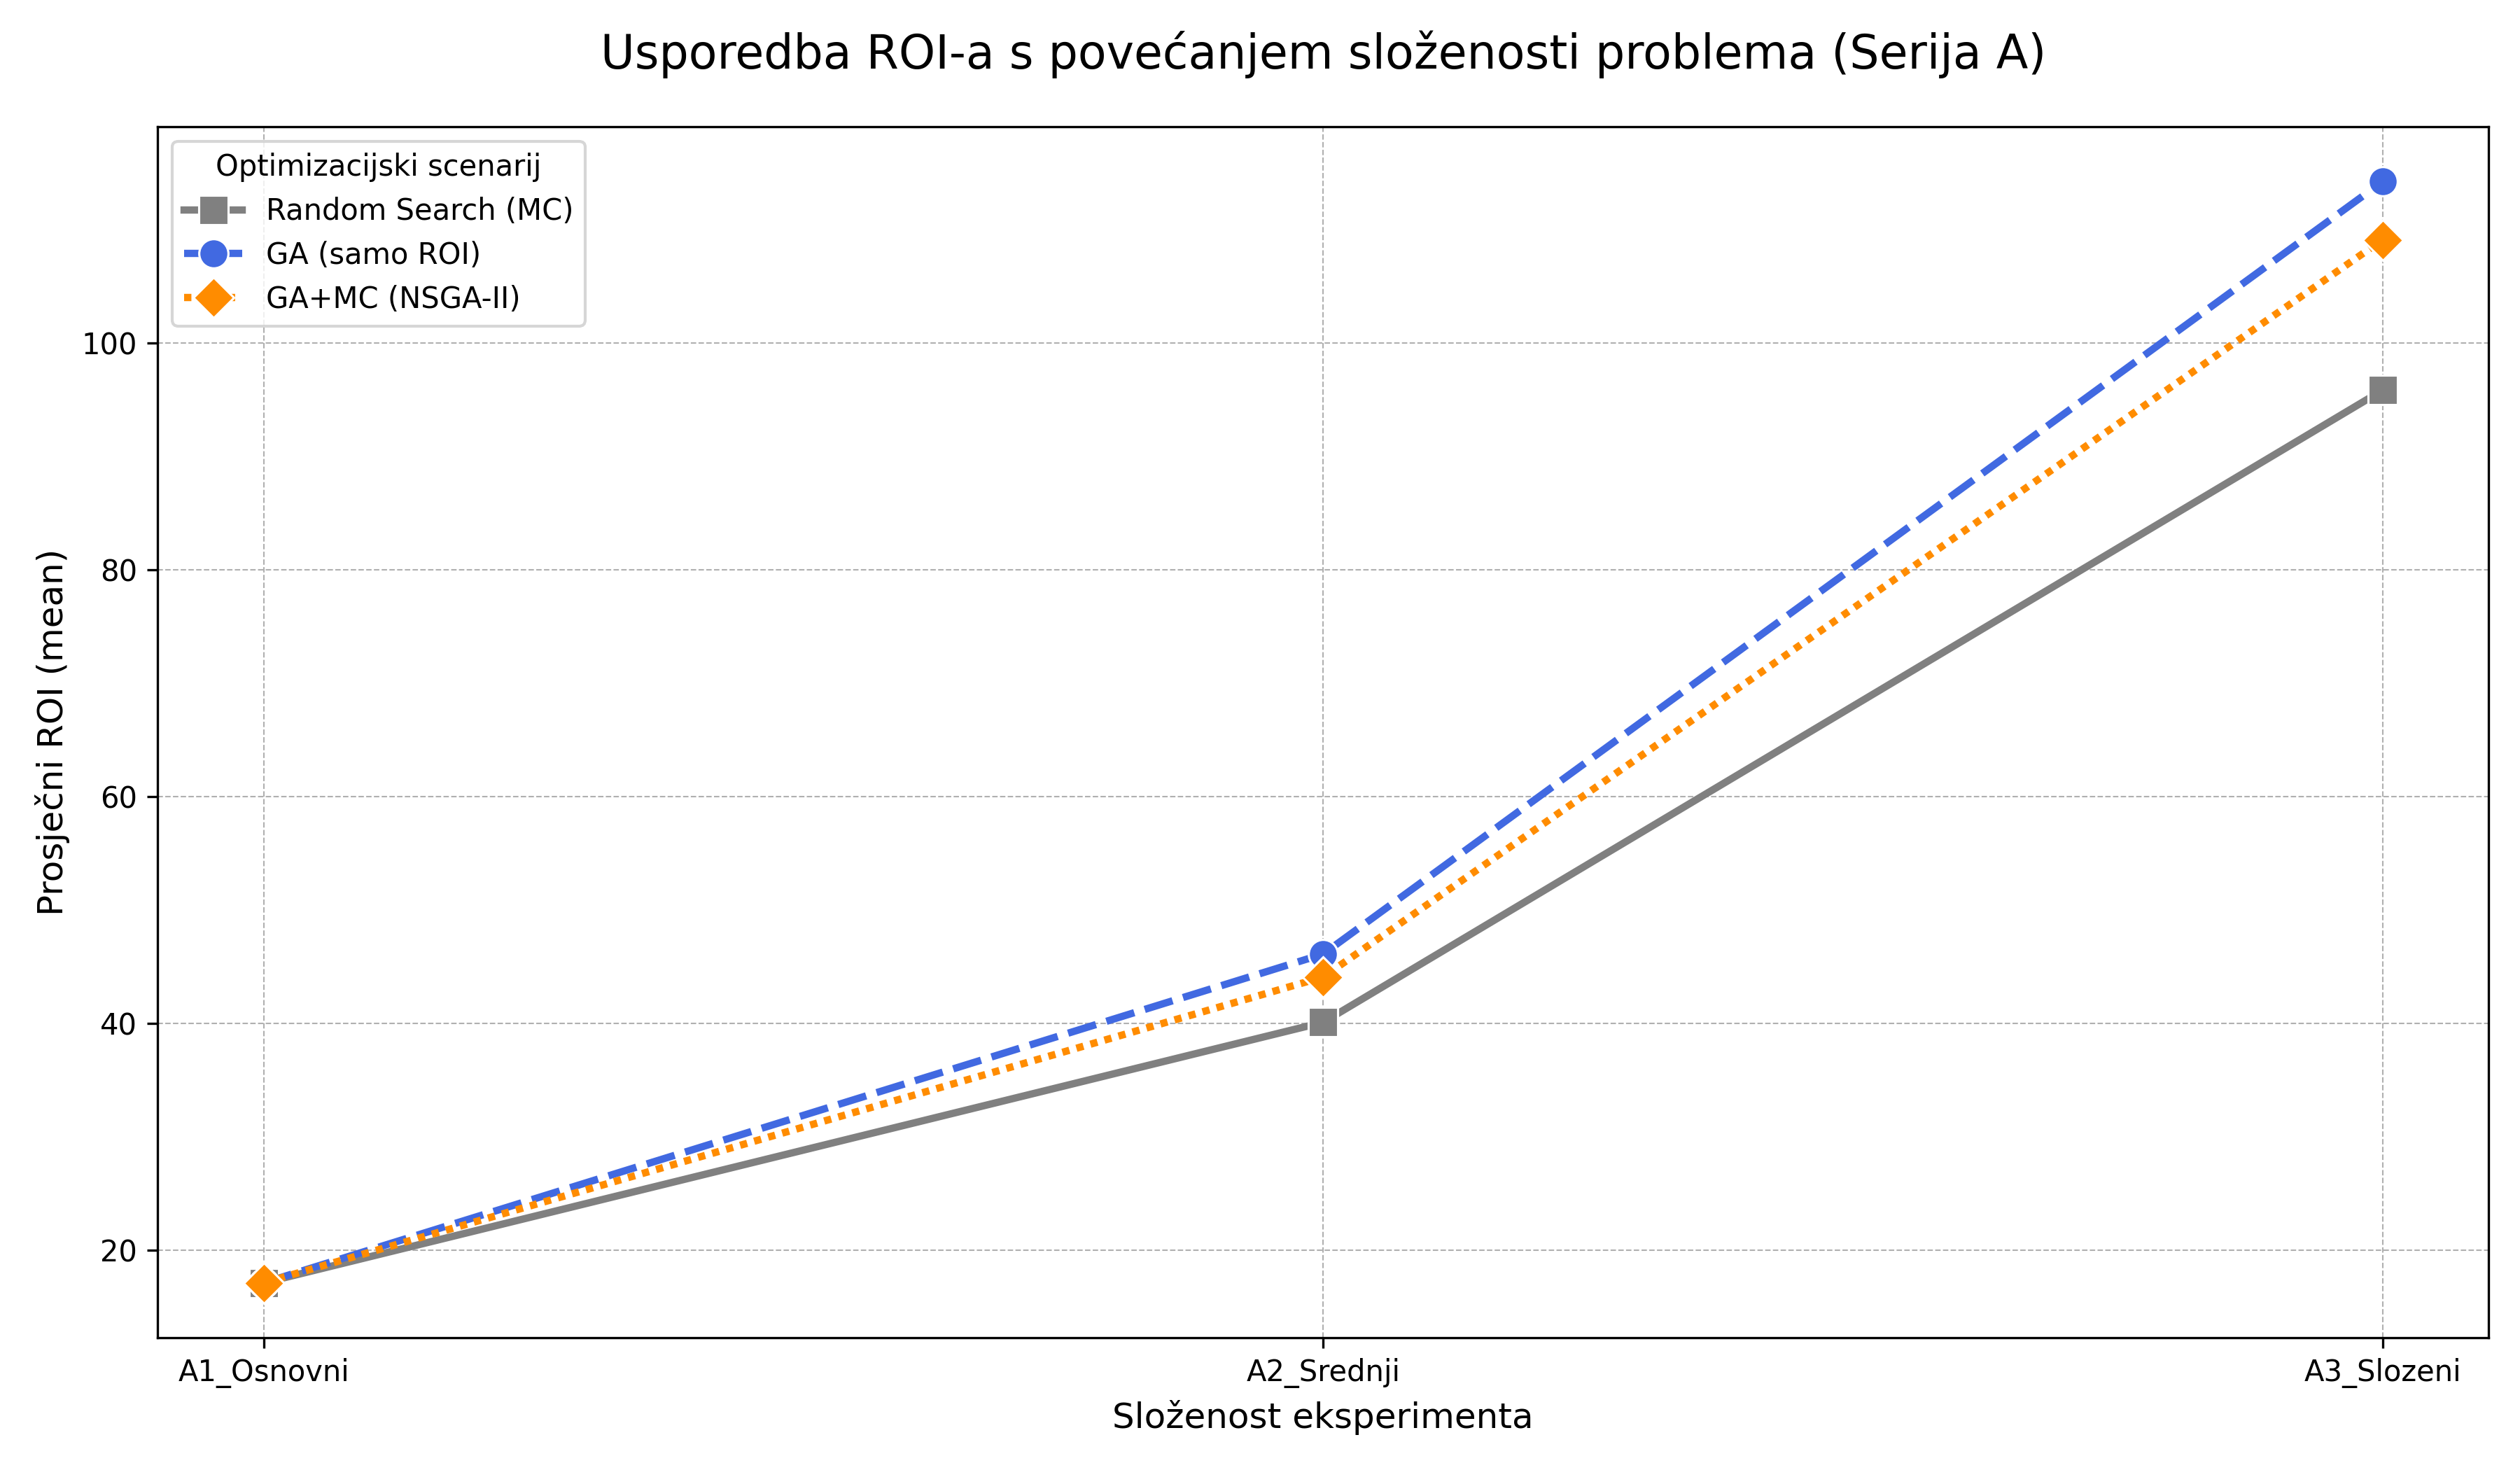
\includegraphics[width=\textwidth]{slike/grafikoni_final/A_skalabilnost_roi.png}
        \caption{Usporedba prosječnog ROI-a.}
    \end{subfigure}
    \hfill
    \begin{subfigure}[b]{0.48\textwidth}
        \centering
        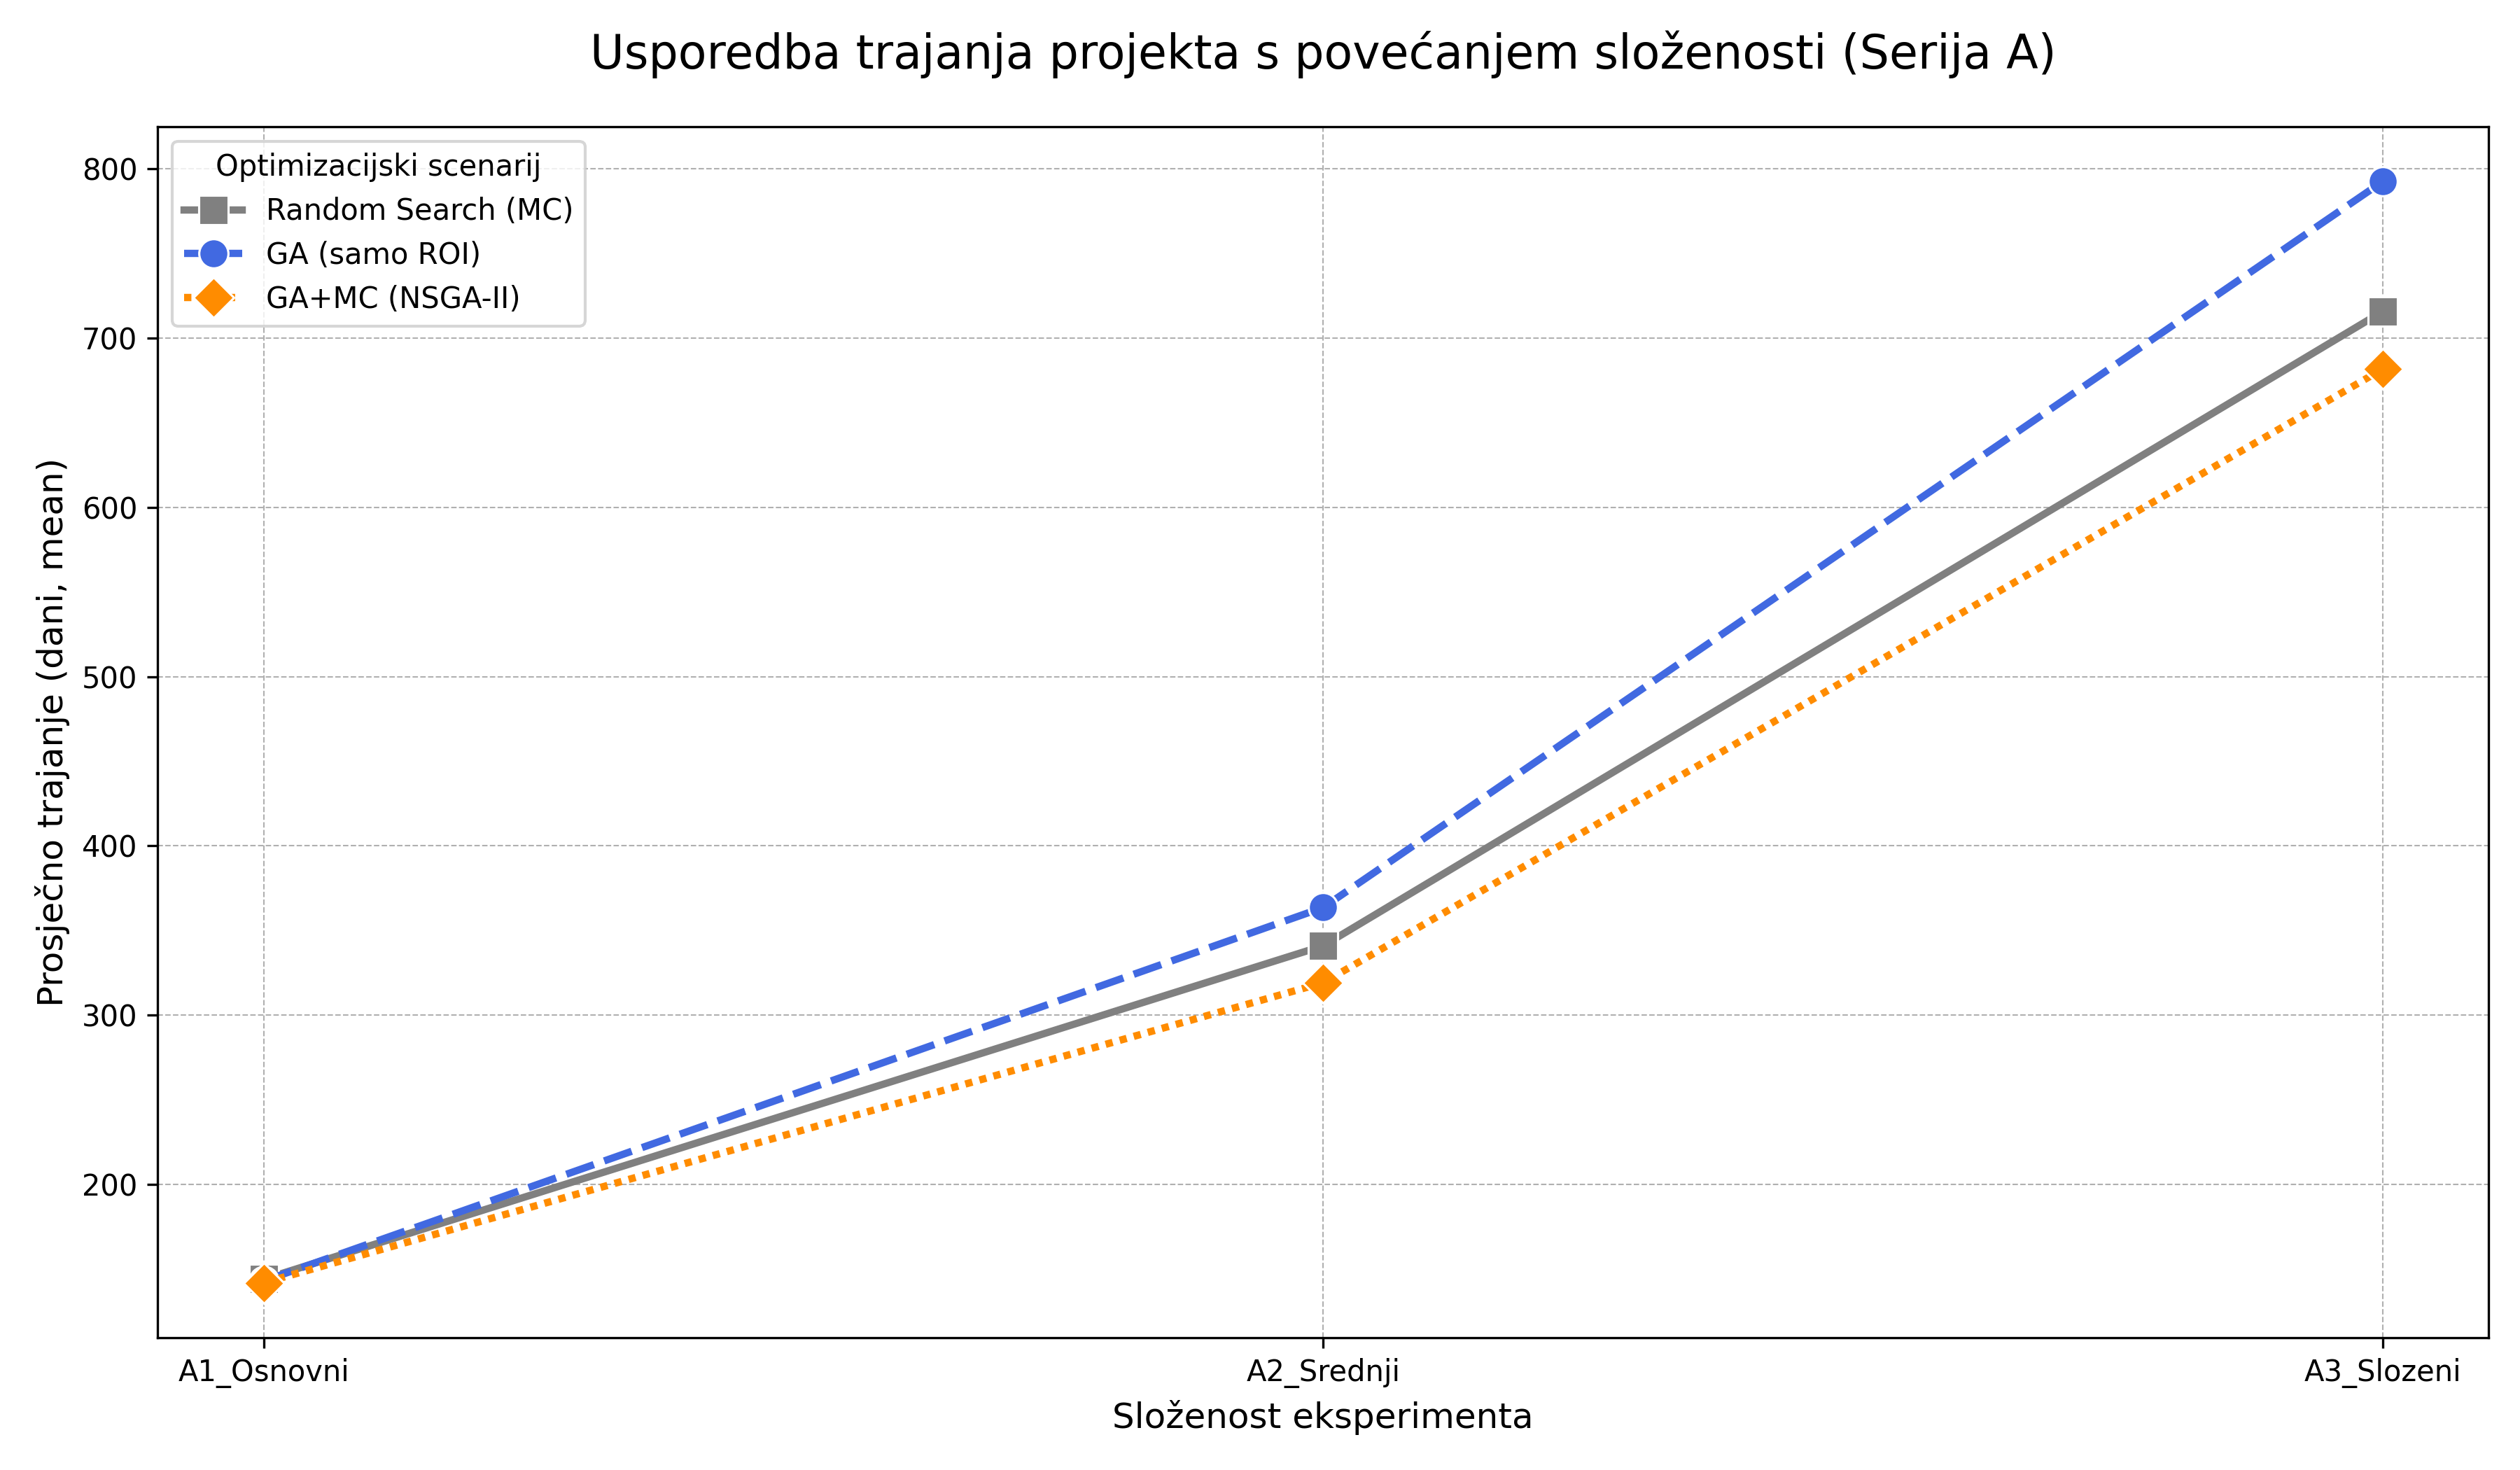
\includegraphics[width=\textwidth]{slike/grafikoni_final/A_skalabilnost_trajanje.png}
        \caption{Usporedba prosječnog trajanja.}
    \end{subfigure}
    \caption{Grafički prikaz rezultata Serije A: Usporedba modela u uvjetima rastuće složenosti.}
    \label{fig:a_skalabilnost}
\end{figure}

\textbf{Analiza Utjecaja Ograničenja (Serija B)}
Slika~\ref{fig:budzet_roi} ilustrira ponašanje modela pod različitim proračunskim pritiskom. Najvažniji nalaz dolazi iz eksperimenta s restriktivnim budžetom (B1), gdje GA+MC (NSGA-II) pokazuje iznimnu krhkost, ne uspijevajući pronaći valjano rješenje u 50\% pokretanja. S druge strane, jednostavniji GA (samo ROI) pokazuje se vrlo robusnim. Ovo ukazuje da složenost više-kriterijske pretrage može biti nedostatak u ekstremno suženim prostorima rješenja. U uvjetima labavog budžeta (B3), svi modeli rade očekivano dobro, potvrđujući hipotezu H3.

\begin{figure}[H]
    \centering
    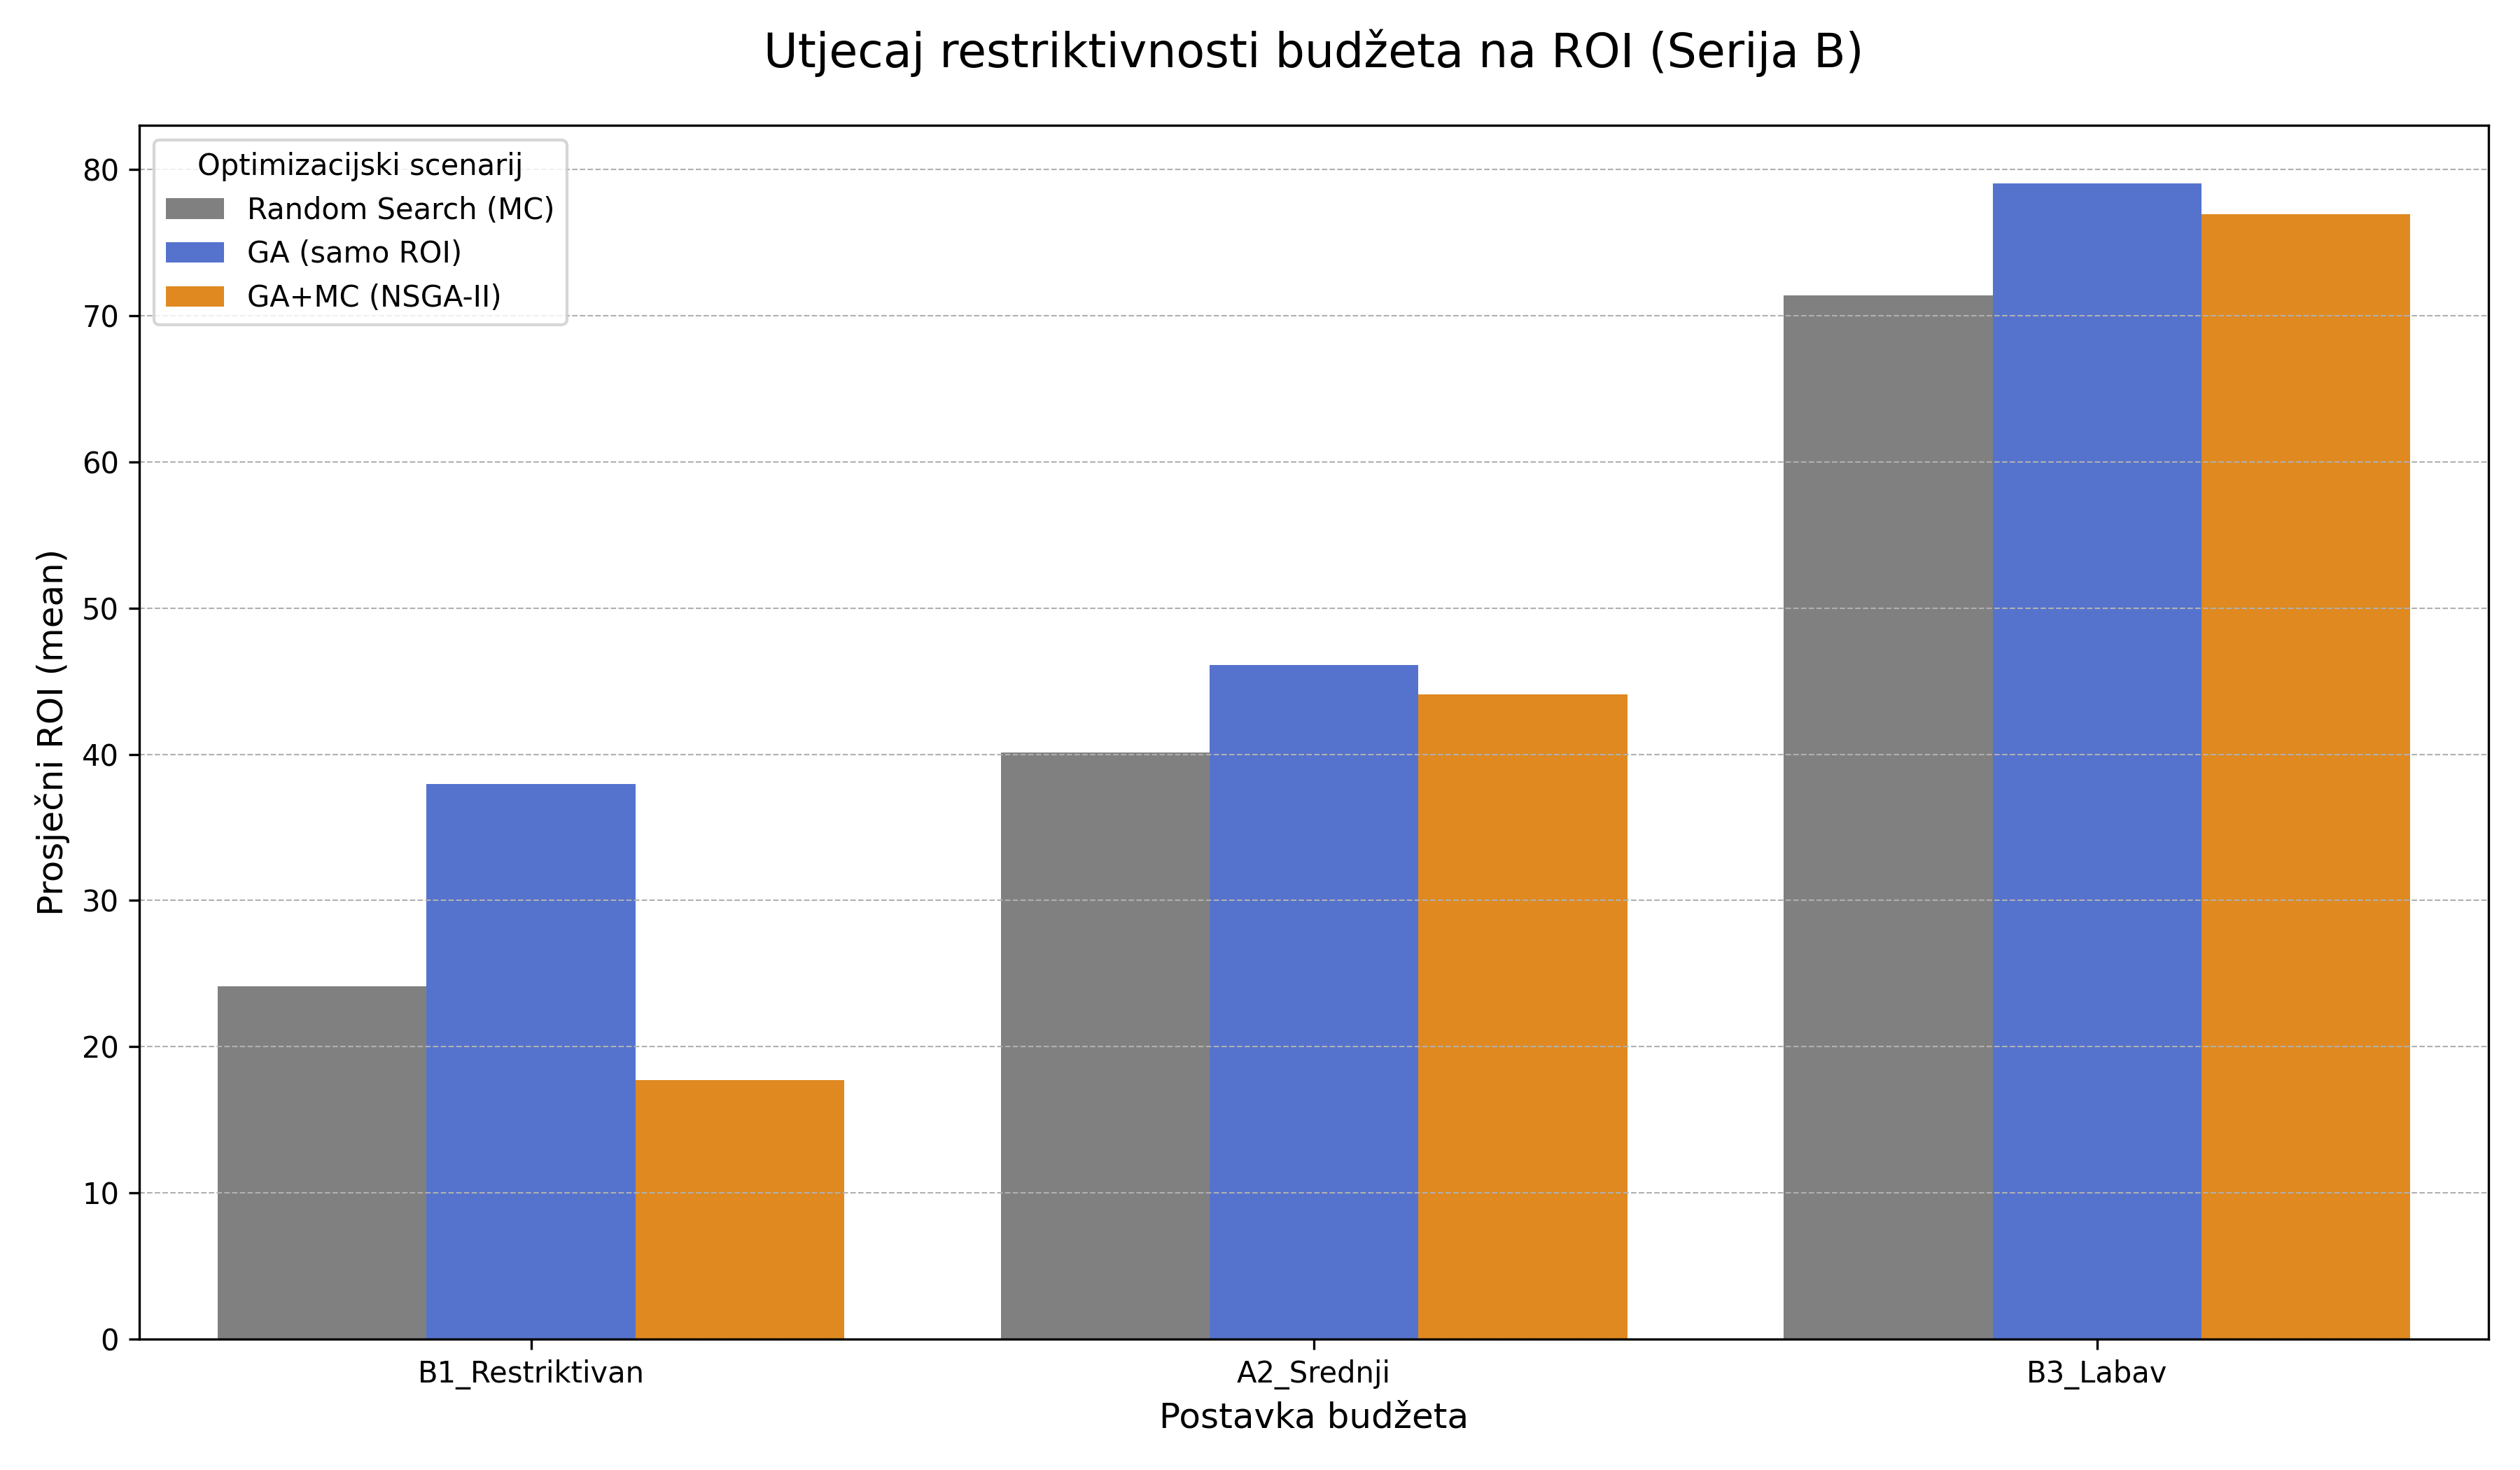
\includegraphics[width=0.8\textwidth]{slike/grafikoni_final/B_budzet_roi.png}
    \caption{Usporedba prosječnog ROI-a modela pod različitim proračunskim ograničenjima (Serija B).}
    \label{fig:budzet_roi}
\end{figure}

\textbf{Analiza Stabilnosti i Pouzdanosti}
Grafikoni na Slici~\ref{fig:stabilnost} prikazuju standardnu devijaciju kao mjeru konzistentnosti. Izvan scenarija B1 gdje je doživio neuspjeh, GA+MC (NSGA-II) model pokazuje usporedivu ili nižu devijaciju trajanja u odnosu na klasični GA. To implicira da rješenja koja nudi nisu samo u prosjeku brža, već su i pouzdanija.

\begin{figure}[H]
    \centering
    \begin{subfigure}[b]{0.48\textwidth}
        \centering
        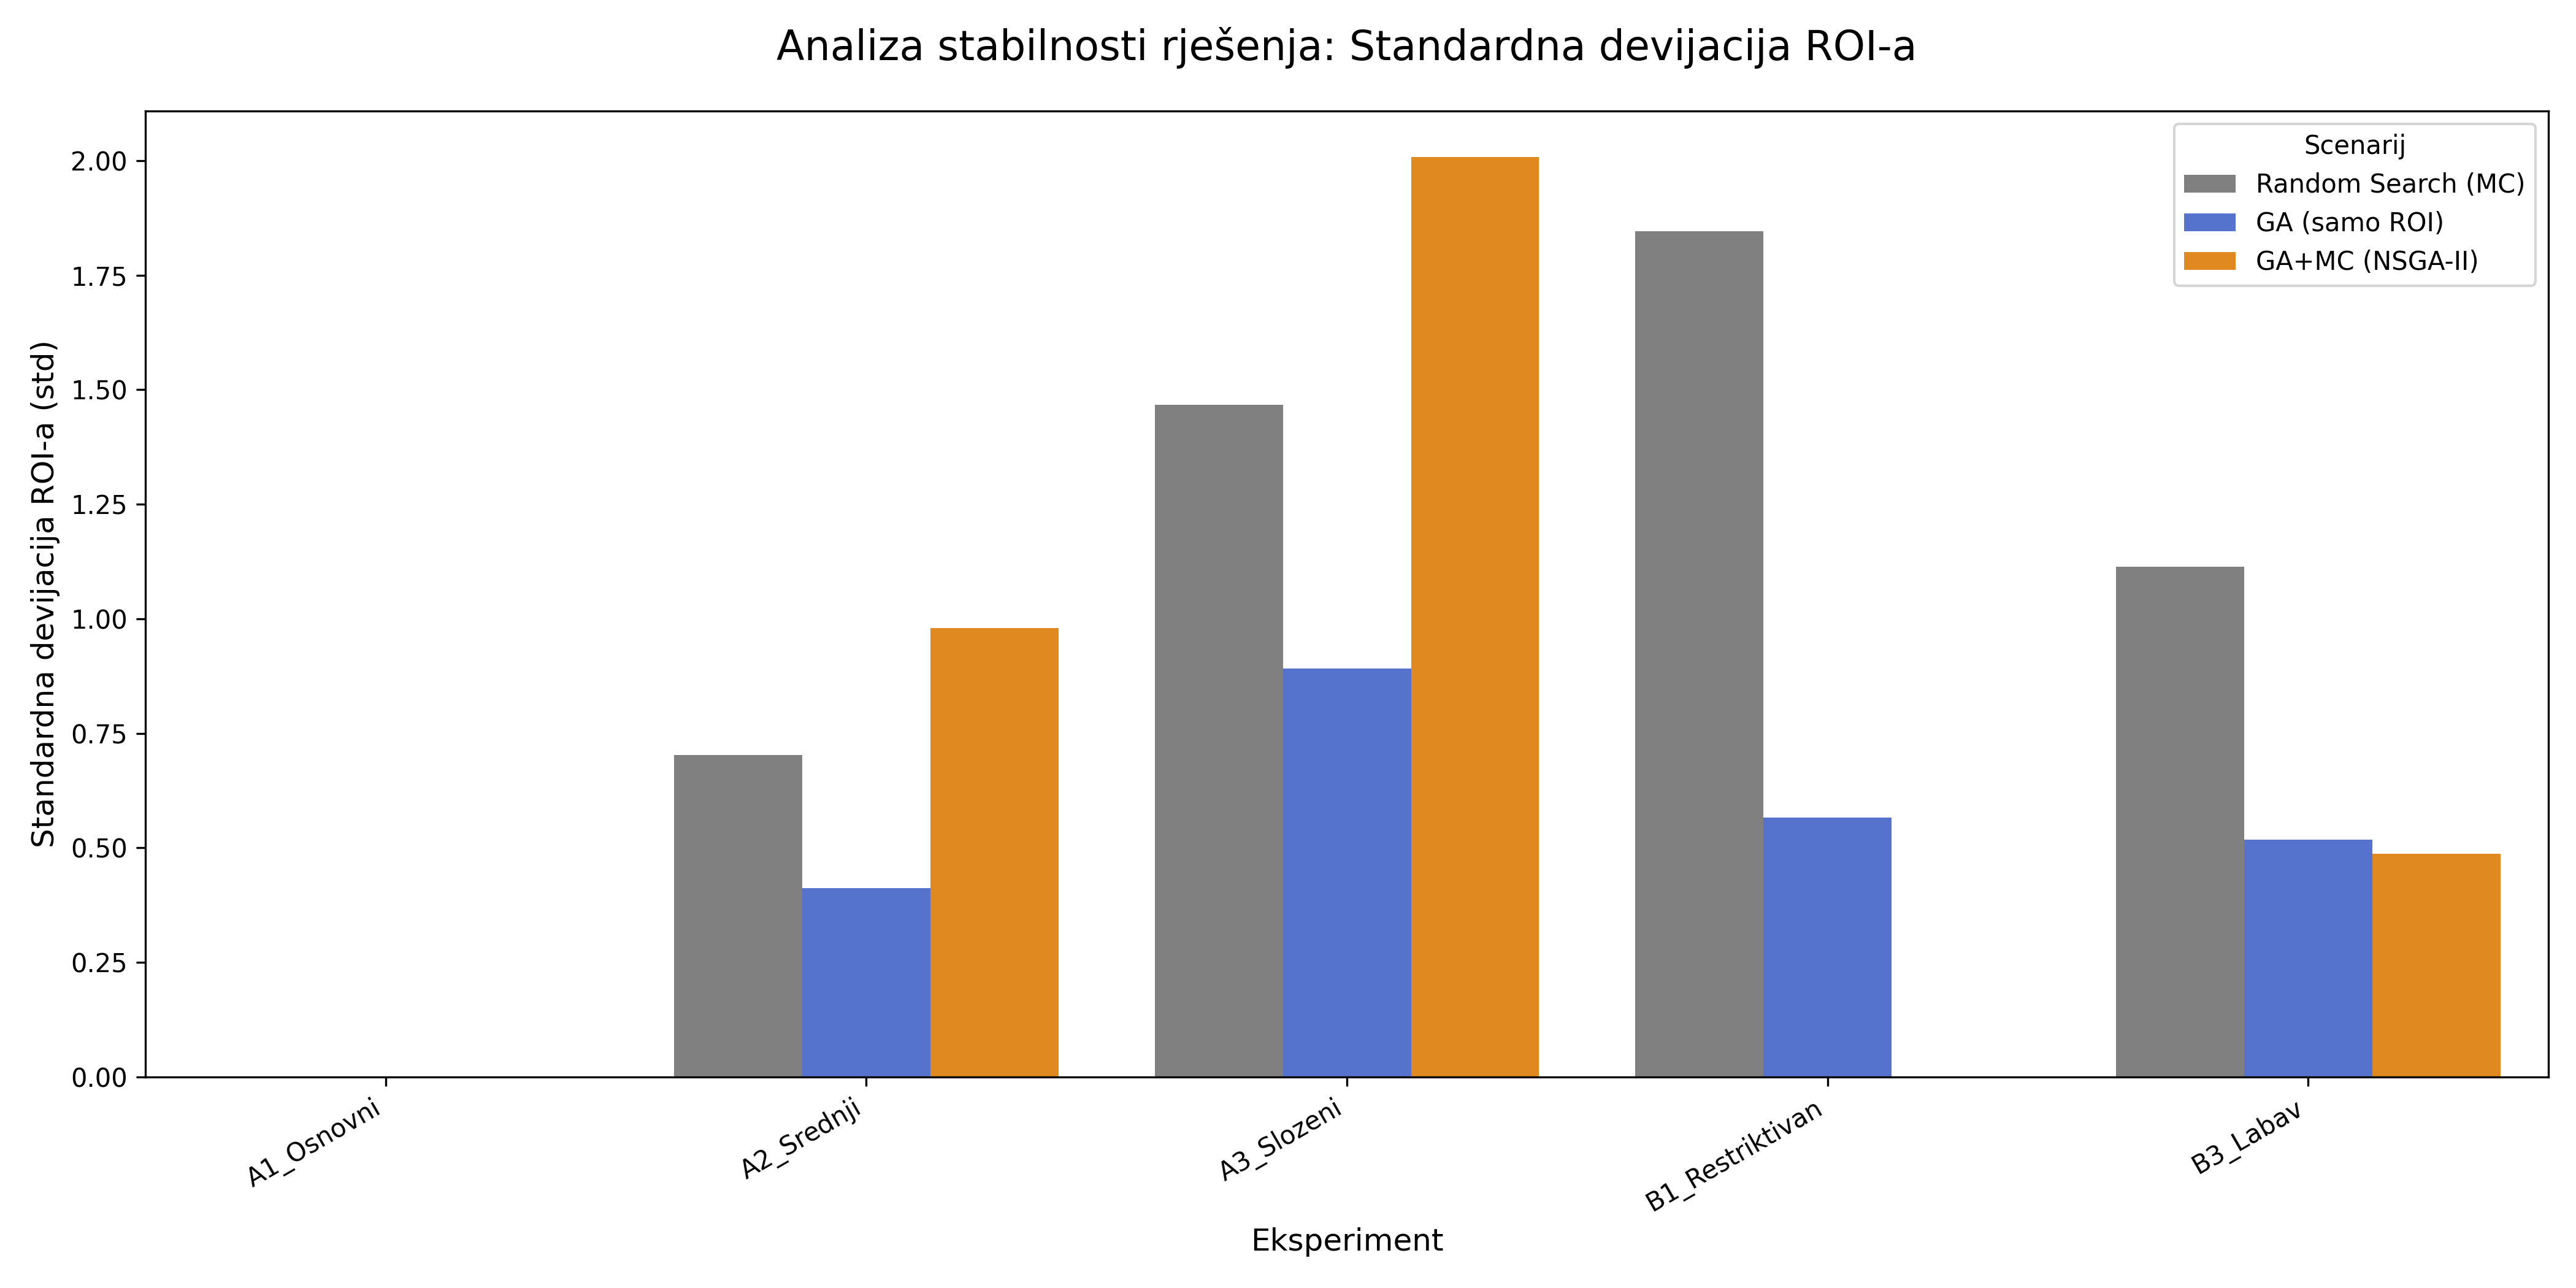
\includegraphics[width=\textwidth]{slike/grafikoni_final/C_stabilnost_roi.png}
        \caption{Stabilnost ROI-a.}
    \end{subfigure}
    \hfill
    \begin{subfigure}[b]{0.48\textwidth}
        \centering
        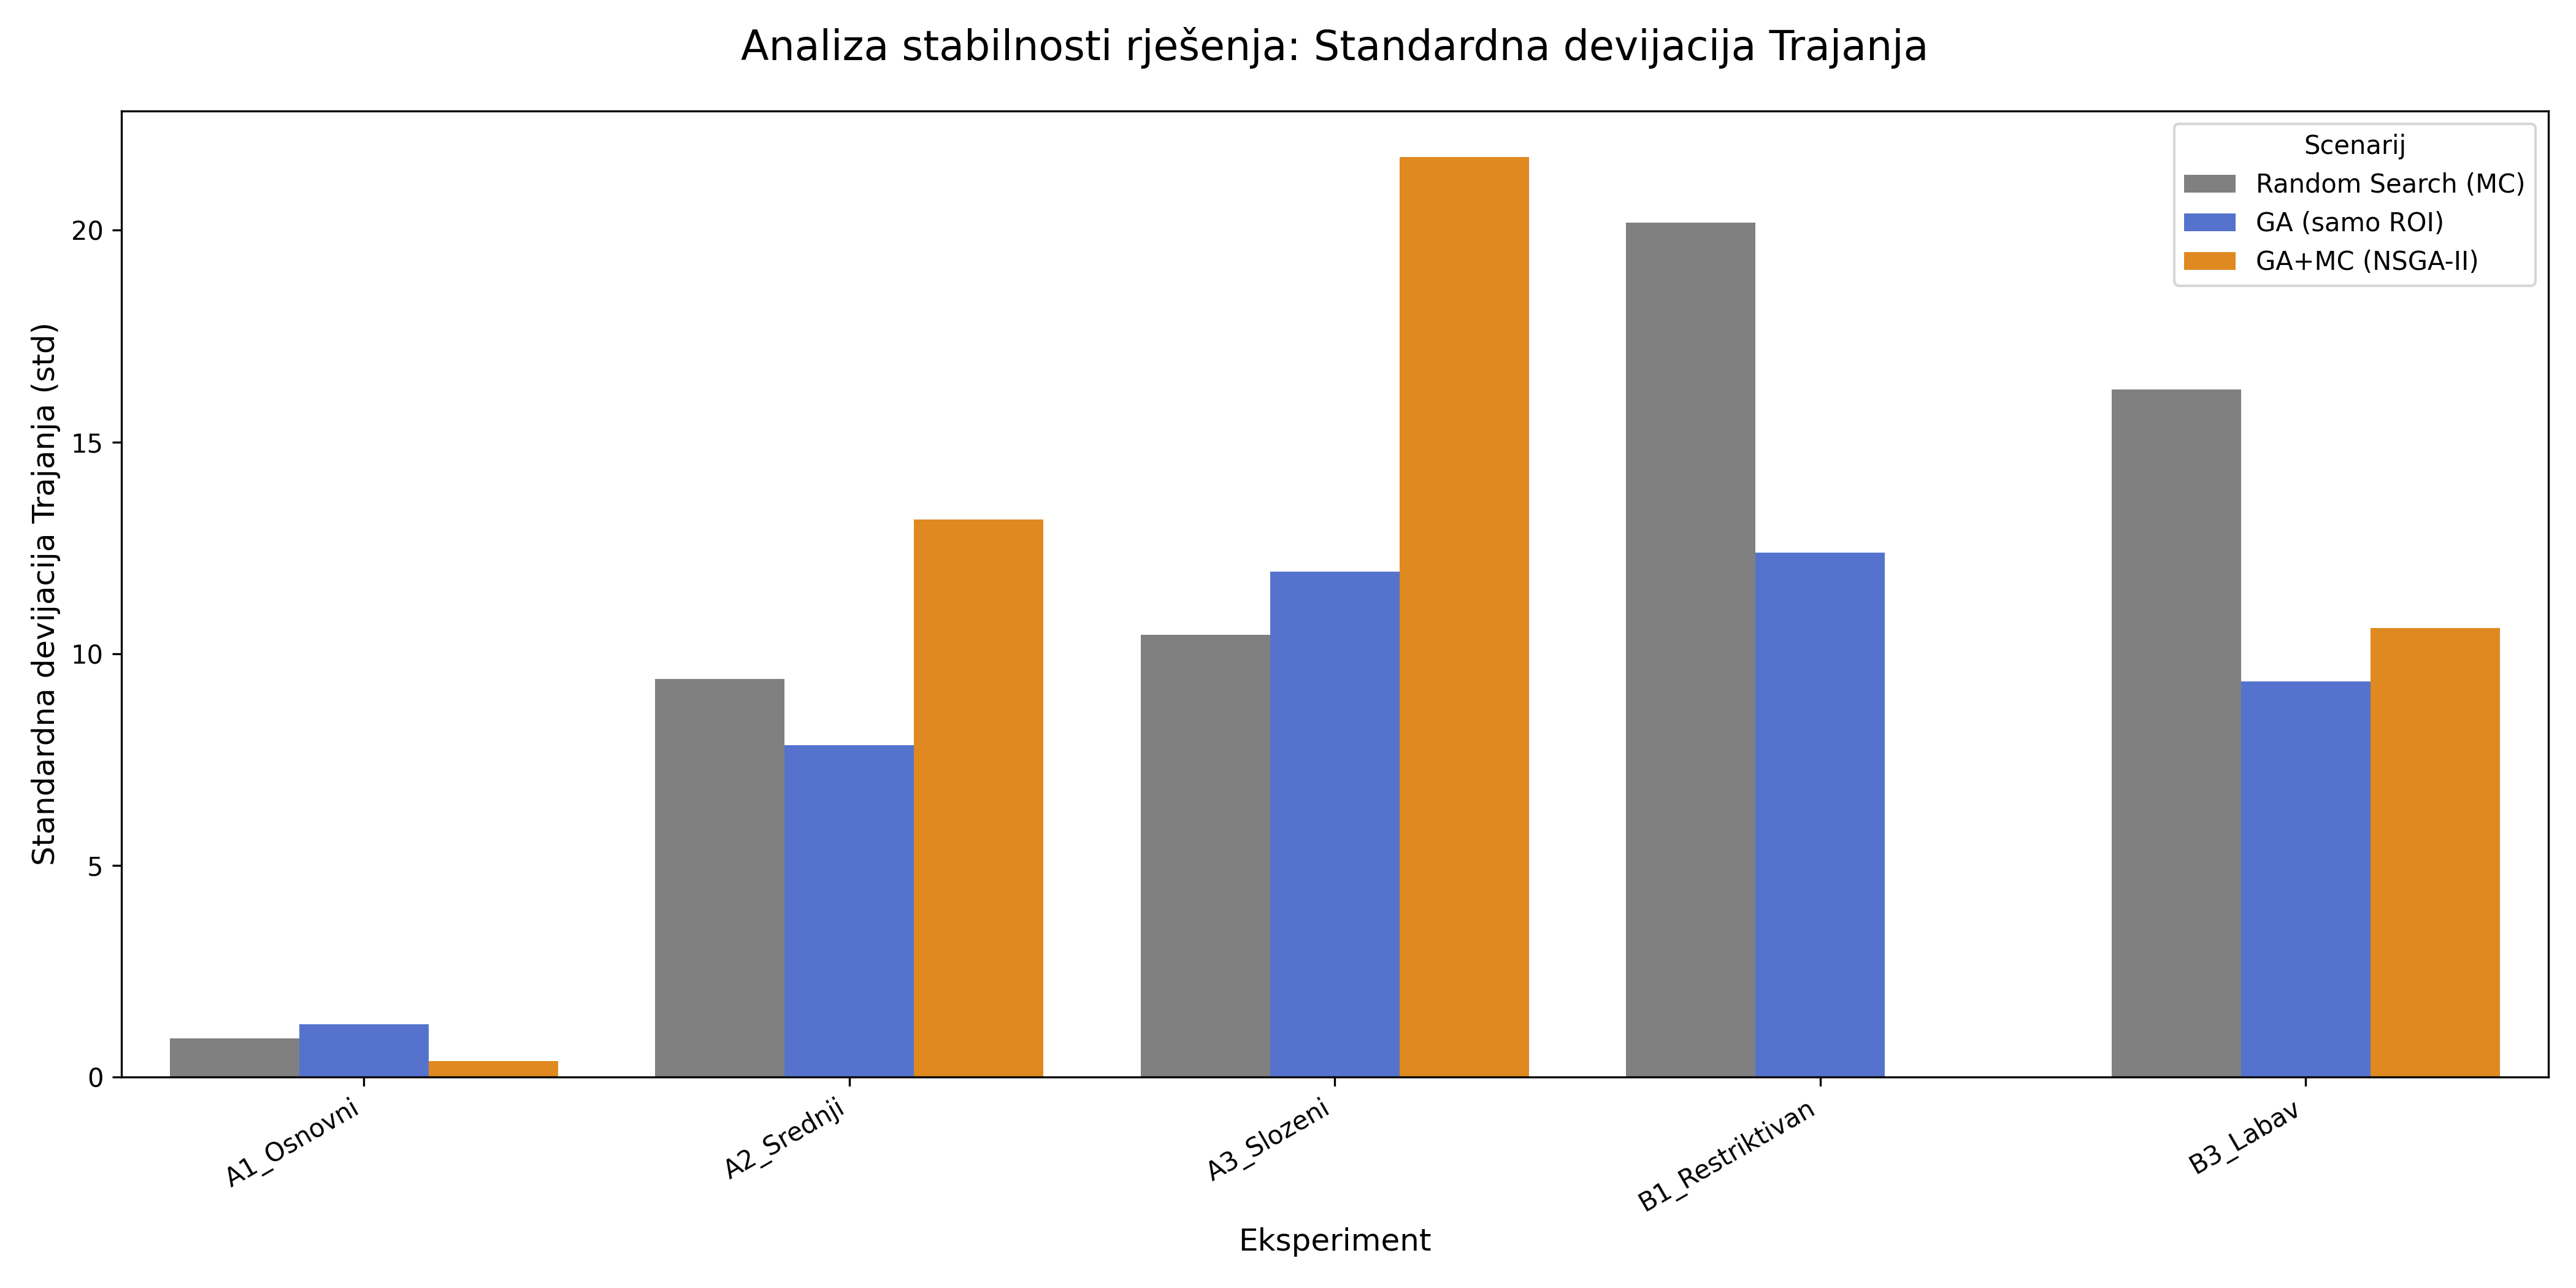
\includegraphics[width=\textwidth]{slike/grafikoni_final/C_stabilnost_trajanje.png}
        \caption{Stabilnost trajanja.}
    \end{subfigure}
    \caption{Grafički prikaz stabilnosti rješenja: Standardna devijacija za ROI i Trajanje.}
    \label{fig:stabilnost}
\end{figure}

\textbf{Dubinska analiza kompromisa: Paretov front}
Raspršeni dijagram na Slici~\ref{fig:pareto_front} pruža dubinski uvid u srž više-kriterijske optimizacije. On prikazuje Paretov front dobiven iz jednog pokretanja GA+MC (NSGA-II) modela na najsloženijem problemu (A3). Svaka točka na grafikonu predstavlja jedno optimalno, ne-dominirano rješenje i ilustrira temeljni kompromis (\emph{trade-off}) između profitabilnosti (Y-os) i rizika trajanja (X-os). Paretov front stoga ne nudi jedno "točno" rješenje, već služi kao strateški alat za donošenje odluka.

\begin{figure}[H]
    \centering
    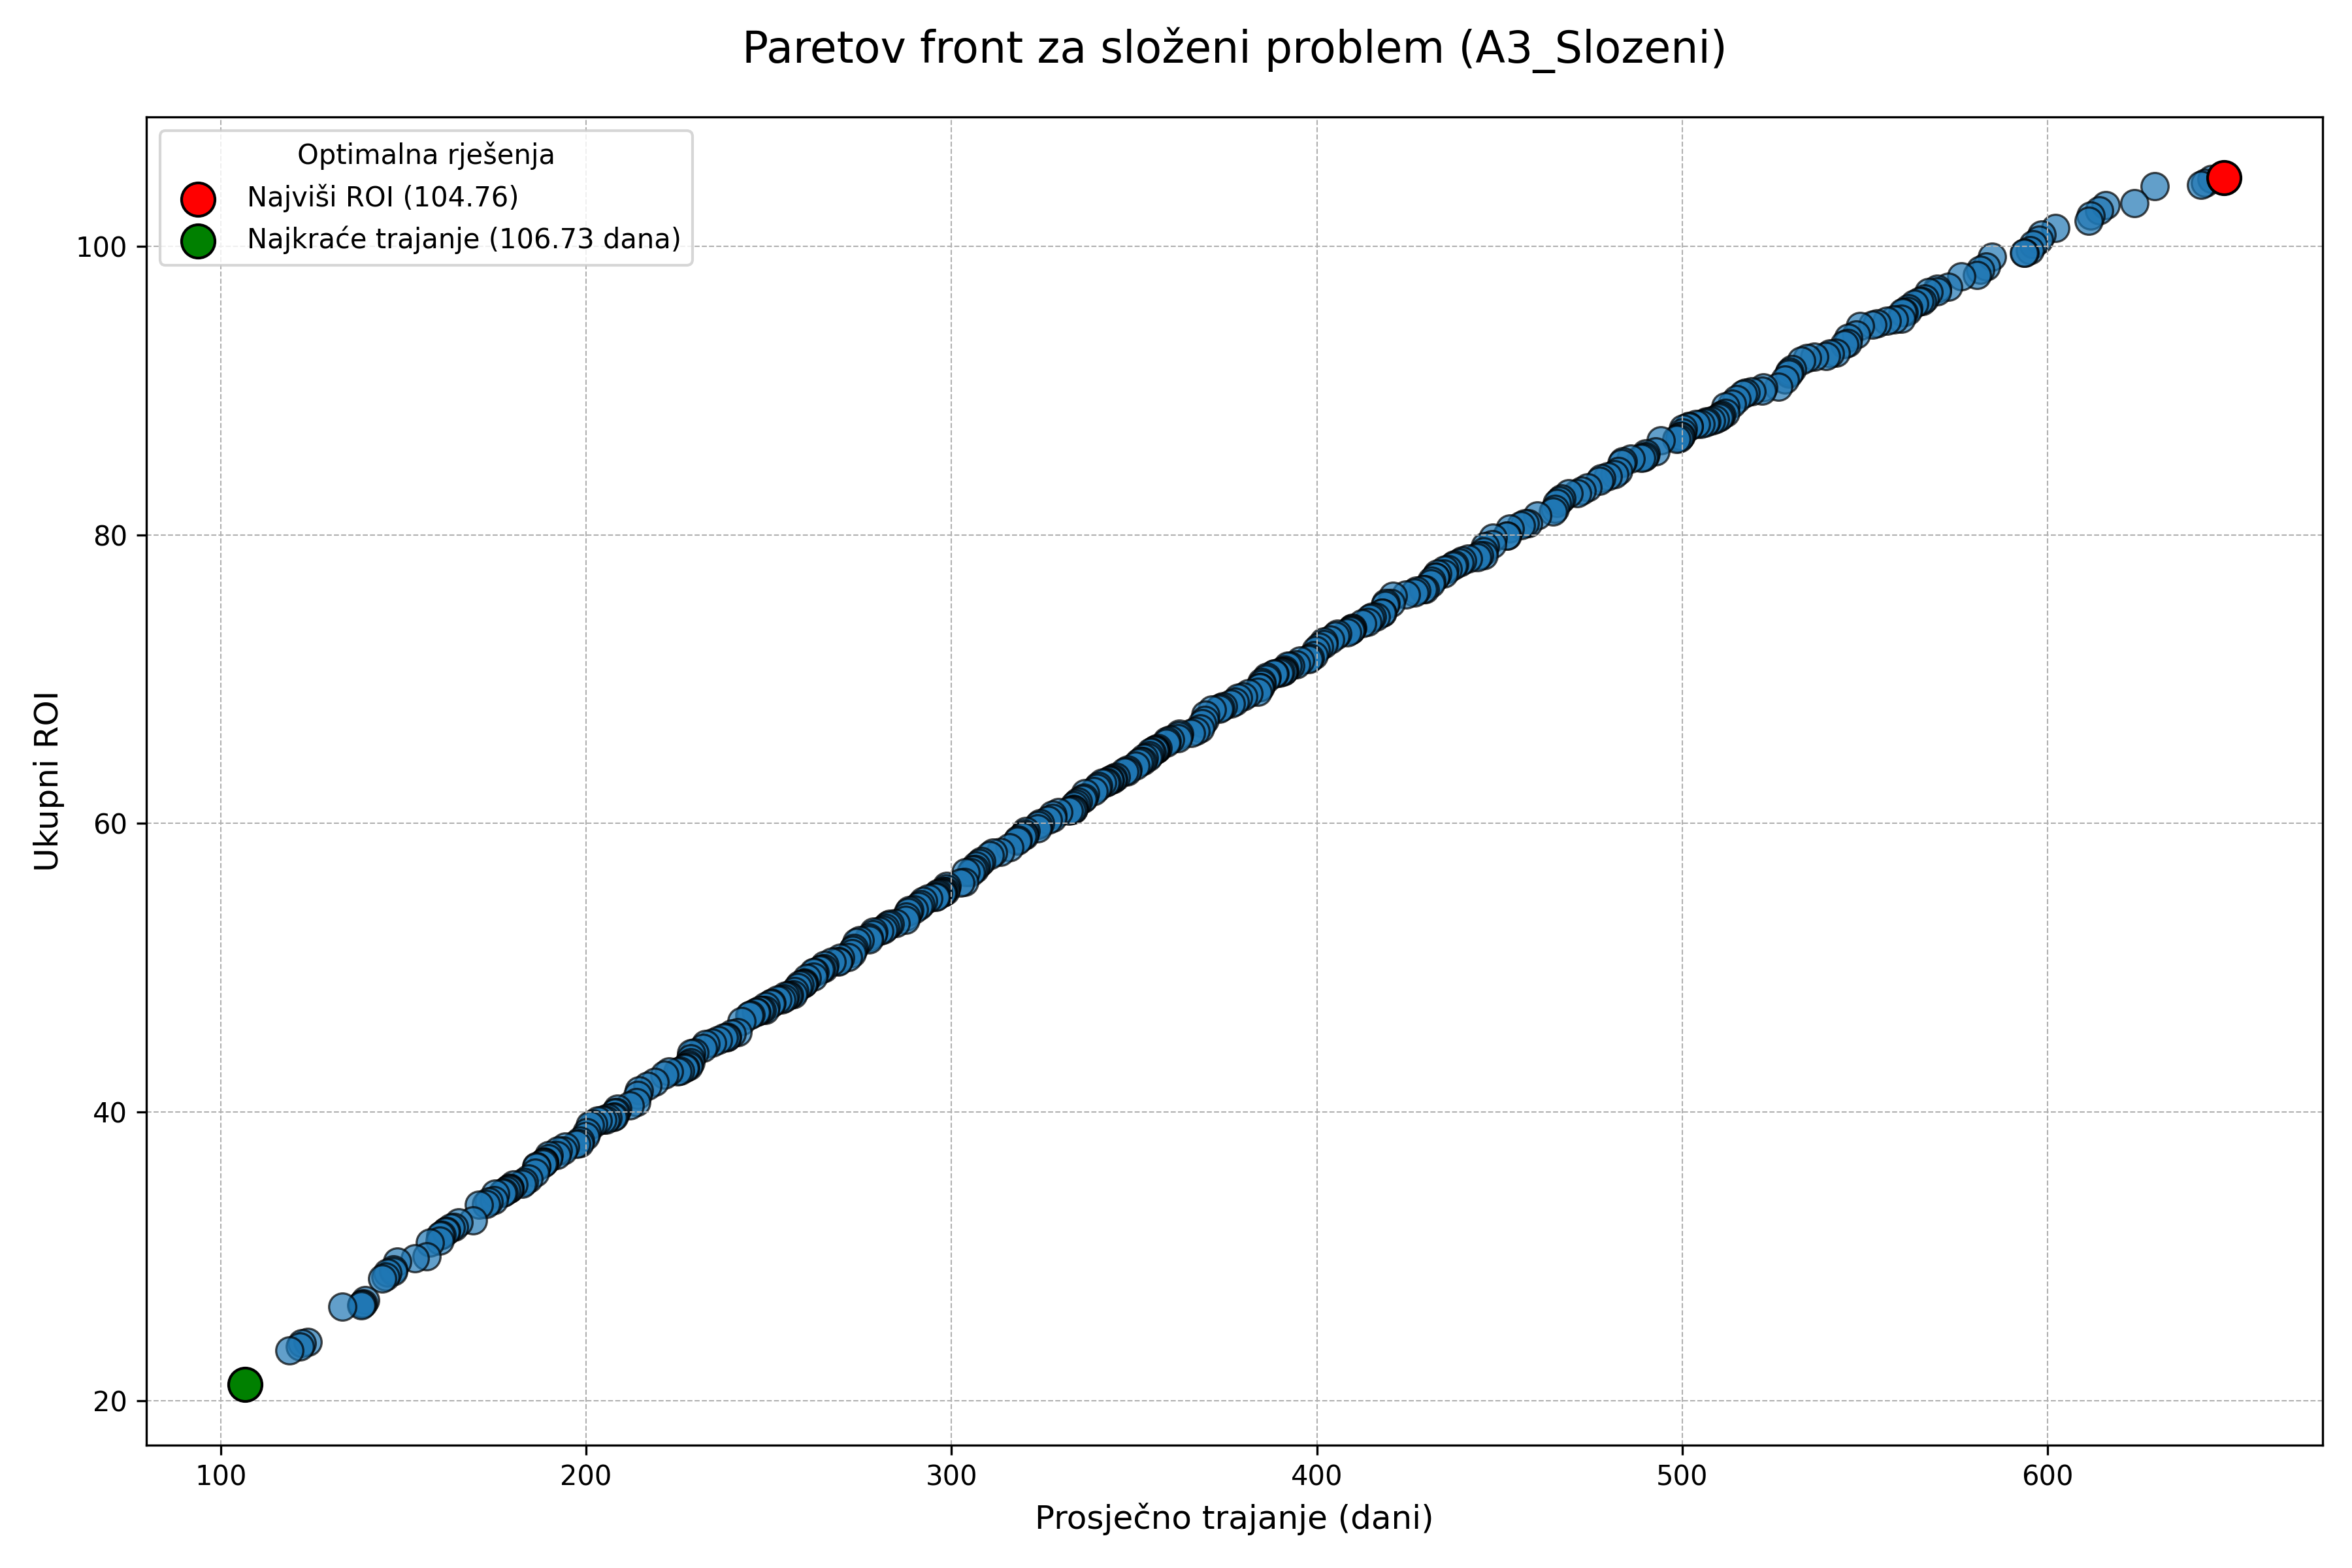
\includegraphics[width=0.9\textwidth]{slike/grafikoni_final/D_pareto_front_scatter.png}
    \caption{Paretov front za složeni problem (A3), koji prikazuje kompromis između ROI-a i trajanja.}
    \label{fig:pareto_front}
\end{figure}

\subsection{Sinteza i interpretacija glavnih nalaza}
Provedeni eksperimenti omogućuju donošenje cjelovitih zaključaka o svakom modelu. Random Search (MC) se pokazao korisnim isključivo kao početna točka na jednostavnim problemima, ali je potpuno neadekvatan kao ozbiljan optimizacijski alat za probleme realne veličine. GA (samo ROI) je izuzetno snažan i robustan "profitni maksimizator", idealan u situacijama gdje je financijska dobit jedini kriterij. Konačno, GA+MC (NSGA-II) je sofisticirani "upravitelj rizikom", čija najveća vrijednost leži u pružanju strateških opcija koje balansiraju profit i rizik. Iako je superioran u standardnim i složenim uvjetima, njegova složenost ga čini osjetljivim u okruženjima s ekstremno restriktivnim ograničenjima.

Konačan izbor modela stoga ovisi o strateškim prioritetima projektnog ureda. Za maksimalan profit, klasični GA je pobjednik. Za uravnoteženo i rizikom informirano donošenje odluka, hibridni GA+MC je superioran, uz nužan oprez pri primjeni u vrlo ograničenim uvjetima.


Nakon detaljne analize pojedinačnih serija eksperimenata, mogu se sintetizirati ključni nalazi koji zajedno oslikavaju cjelovitu sliku o performansama, prednostima i nedostacima svakog od testiranih optimizacijskih modela. Interpretacija ovih nalaza pruža direktne odgovore na postavljene istraživačke hipoteze.

Potvrda superiornosti genetskih algoritama (H1):
Prvi i najjasniji zaključak jest da je hipoteza o skalabilnosti (H1) u potpunosti potvrđena. Iako je Random Search metoda, zbog velikog broja evaluacija, uspijevala pronaći valjana rješenja, njezina učinkovitost nije pratila eksponencijalni rast složenosti problema. S druge strane, oba genetska algoritma pokazala su sposobnost inteligentno vođene pretrage, konzistentno pronalazeći značajno superiornija rješenja. Za projektnog menadžera, praktična implikacija je nedvosmislena: za bilo koji netrivijalan problem odabira portfelja, primjena metaheurističkih metoda poput genetskih algoritama nije samo poboljšanje, već nužnost za postizanje konkurentnih rezultata.

Kvantifikacija kompromisa između profita i rizika (H2):
Središnji nalaz istraživanja proizašao je iz usporedbe dvaju genetskih algoritama. Model GA (samo ROI) se dokazao kao iznimno učinkovit "profitni maksimizator", konzistentno pronalazeći rješenja s najvišim mogućim povratom na investiciju. Međutim, bio je potpuno "slijep" na rizik trajanja, često birajući portfelje s dugim i nepredvidljivim vremenom izvođenja.

Tu do izražaja dolazi ključni doprinos hibridnog GA+MC (NSGA-II) modela. Njegova svrha nije bila nadmašiti klasični GA u jednoj dimenziji (ROI), već otkriti i kvantificirati sam kompromis između profitabilnosti i rizika, čime je potvrđena hipoteza H2. Kao što rezultati i Paretov front (Slika~\ref{fig:pareto_front}) pokazuju, hibridni model omogućuje donošenje strateške odluke. On kvantificira "cijenu" smanjenja rizika, pokazujući, primjerice, da se za 5-10% niži ROI može dobiti portfelj koji je 15-25% brži i, što je još važnije, statistički pouzdaniji. Za donositelja odluka, ovo transformira optimizacijski problem iz potrage za jednim brojem u sofisticirani alat za strateško planiranje.

Otkriće o robusnosti i krhkosti modela (H3):
Konačno, analiza utjecaja ograničenja (Serija B) potvrdila je hipotezu H3 i dovela do najdubljeg i pomalo neočekivanog zaključka. Dok je klasični GA (samo ROI) pokazao iznimnu robusnost, pronalazeći dobra rješenja čak i pod vrlo restriktivnim budžetom, napredni GA+MC (NSGA-II) model pokazao je neočekivanu krhkost. Njegov složeni, više-kriterijski mehanizam pretrage, koji briljira u velikim i otvorenim prostorima rješenja, postao je njegova slabost u ekstremno suženom prostoru valjanih opcija, što je dovelo do čestih neuspjeha.

Ovaj nalaz nosi ključnu praktičnu poruku: tehnološki najnapredniji alat nije uvijek najbolji alat za svaku situaciju. U kriznim scenarijima s ekstremno ograničenim resursima, jednostavniji i fokusiraniji pristup može biti pouzdaniji.

Za lakši pregled, konačna ocjena svakog modela sažeta je u Tablici~\ref{tab:sinteza_modela}.


\begin{table}[H]
\centering
\caption{Sintetička usporedba evaluiranih modela.}
\label{tab:sinteza_modela}
\resizebox{\textwidth}{!}{
\begin{tabular}{|l|l|l|}
\hline
\textbf{Model} & \textbf{Najbolji za...} & \textbf{Ključna ograničenja} \\
\hline
\textbf{Random Search (MC)} & Postavljanje osnovne linije (baseline) na jednostavnim problemima. & Potpuno neefikasan i nepouzdan na složenim problemima. \\
\hline
\textbf{GA (samo ROI)} & Scenarije gdje je maksimizacija profita jedini i isključivi cilj. & Zanemaruje rizik trajanja; može predložiti vrlo duge projekte. \\
\hline
\textbf{GA+MC (NSGA-II)} & Strateško odlučivanje; balansiranje između profita i rizika. & Računalno zahtjevan; nepouzdan u ekstremno restriktivnim uvjetima. \\
\hline
\end{tabular}
}
\end{table}
Konačan izbor modela stoga ovisi o strateškim prioritetima projektnog ureda. Za maksimalan profit, klasični GA je pobjednik. Za uravnoteženo i rizikom informirano donošenje odluka, hibridni GA+MC je superioran, uz nužan oprez pri primjeni u vrlo ograničenim uvjetima.
